
%Vectors and Basis vectors
\renewcommand{\vec}[1]{\mathbf{#1}}

\newcommand{\eet}{\vec{e}_1}
\newcommand{\eto}{\vec{e}_2}
\newcommand{\etr}{\vec{e}_3}
\newcommand{\eets}{\eet\cdot\eet}
\newcommand{\etos}{\eto\cdot\eto}
\newcommand{\eetto}{\eet\cdot\eto}

\newcommand{\vc}[3]{
  \left( \begin{array}{c}
  #1 \\ #2 \\ #3
  \end{array} \right)
}

% Derivatives
\newcommand{\dvd}[2]{\partial\vec{#1}/\partial#2}

\newcommand{\dd}[2]{\frac{\partial #1}{\partial #2}}

\newcommand{\drdt}{\dvd{r}{\theta}}
\newcommand{\drdp}{\dvd{r}{\phi}}


% Trigonometric
\newcommand{\stsp}{\sin\theta\sin\phi}
\newcommand{\stcp}{\sin\theta\cos\phi}
\newcommand{\ctsp}{\cos\theta\sin\phi}
\newcommand{\ctcp}{\cos\theta\cos\phi}
\newcommand{\st}{\sin\theta}
\newcommand{\ct}{\cos\theta}
\newcommand{\sip}{\sin\phi}
\newcommand{\cop}{\cos\phi}

% Editorial
\newcommand{\url}[1]{\mbox{\textbf{#1}}}
\newcommand{\wiki}[1]{#1}
\newcommand{\command}[1]{\$ \textbf{#1}}
\newcommand{\addformula}[1]{
\vspace{0.5cm}
\fbox{Add: #1}
\vspace{0.5cm}
}
\newcommand{\fixme}[1]{
\vspace{0.5cm}
\fbox{#1}
\vspace{0.5cm}
}
\newcommand{\myhrule}{\rule{\linewidth}{0.5pt}}


% TikZ macros
\newcommand{\TikZ}{Ti\emph{k}Z~}
\newcommand{\fsz}{\fontsize{12}{12}}

\newcommand{\txfig}[4]{
    \clip (#1-0.4,#2-0.4) rectangle (#3 + 0.4,#4 +0.4 );
    \draw[step=.25cm,mjcgrid] (#1-0.4,#2-0.4) grid (#3 + 0.4,#4 +0.4 );
    \pgfsetlinewidth{1pt}

    \coordinate (o)  at ( 0, 0);
    \coordinate (bx) at (#1, 0);
    \coordinate (by) at ( 0,#2);
    \coordinate (ex) at (#3, 0);
    \coordinate (ey) at ( 0,#4);
    \draw [->] (bx) -- (ex); 
    \draw [->] (by) -- (ey); 

    \node [right]  at (ex) {$x$};
    \node [above]  at (ey) {$y$};
    \foreach \x in {#1,...,#3} \draw[black!70] (\x cm,1pt) -- (\x cm,-1pt) node[anchor=north] {$\x$};
    \foreach \y in {#2,...,#4} \draw[black!70] (1pt,\y cm) -- (-1pt,\y cm) node[anchor=east]  {$\y$};
}


\newenvironment{example}{%
   \vspace{5mm}
   \noindent\ignorespaces%
    \textbf{Example:}\ }
{\par\noindent% 
     \ignorespacesafterend}


\newcommand{\var}[3]{
   \left( \begin{array}{ccc}
   #1 \\ #2 \\ #3
   \end{array} \right)
}

\newcommand{\myindx}[1]{\index{#1}#1}


\newenvironment{wide}{%
   \fontsize{6}{8}
  \let\oldmarginparwidth\marginparwidth 
  \setlength{\marginparwidth}{0pt}%
}{%
  \setlength{\marginparwidth}{\oldmarginparwidth}%
}

\newenvironment{twocol}[2]{%
\begin{minipage}{0.5\linewidth}
#1
\end{minipage}
\begin{minipage}{0.5\linewidth}
#2
\end{minipage}
}
{}


%\includeonly{vectors}
%\includeonly{coordsys}
%\includeonly{maps}
%\includeonly{2dcurves}
%\includeonly{3dcurves}
%\includeonly{curvature_I}
%\includeonly{curvature_II}
%\includeonly{tangents}
%\includeonly{4dcurves}
%\includeonly{parallel}
%\includeonly{maxima}
%\includeonly{people}
%\includeonly{refs}

\documentclass[a4paper,openany,10pt]{memoir}
\chapterstyle{bianchi}
\usepackage[ISBN=978-87-994778-1-4]{ean13isbn}
\usepackage{makeidx}
\usepackage{auto-pst-pdf}
\usepackage{xcolor}
\usepackage{color}
%\usepackage{fancyhdr}
\setlength{\headheight}{15pt}
\usepackage{graphicx,ifthen,amsmath,listings,tikz}
\usepackage{amsthm}
\usepackage{pstricks}
\usepackage{pst-3dplot}
\usepackage{pst-solides3d}

\theoremstyle{remark} % Removes italic from example text 
\newtheorem{myex}{Example}[chapter]

\makeindex
%\pagestyle{fancy}
\renewcommand{\chaptermark}[1]{%
    \markboth{#1}{}} 
\renewcommand{\sectionmark}[1]{%
    \markright{\thesection\ #1}}

% TikZ Styles and Modules
\tikzset{mjcgrid/.style={help lines,color=blue!20}}
\usetikzlibrary{calc}


% Document
\begin{document}
\enlargethispage{3\baselineskip}
\thispagestyle{empty}
{
\pagecolor[HTML]{660066}
\color{white}\Large\bfseries

\vspace*{\droptitle}
\begin{flushright} \Large \lineskip 0.5em
     Morten Jagd Christensen \par
\end{flushright}

\begin{center} \HUGE \sffamily
Mathematics of Curves and Surfaces
  \par 
\end{center}

\vspace{2cm}

%\begin{figure}
%\input{figures/trefoil.eps}
%\end{figure}

  \begin{figure}[htb]
    \begin{center}
      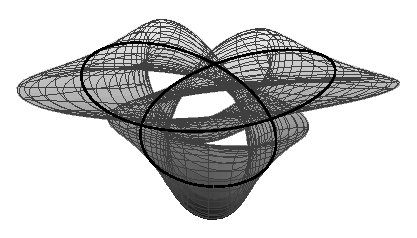
\includegraphics[width=12cm,height=12cm]{figures/trefoil}
    \end{center}
  \end{figure}

\vspace*{\baselineskip}

\begin{center}
  \Large \textsf{jCAPS Publishing \textbullet\ Autumn 2010}
\end{center}
}

  \clearpage
  \pagecolor[HTML]{FFFFFF}
  \color{black}
  \tableofcontents
  \chapter{Introduction}

æøåÆØÅ

I began writing this document as a side effect of trying to understand General Relativity, which makes 
heavy use of \myindx{differential geometry}.

Here I will show some examples of 2D surfaces embedded in 3D euclidian spaces, how to create 
curves on these surfaces and how to evaulate the length of these curves. The necessary 
mathematics is introduced but the reader is assumed to be familiar with vectors, matrices and 
\myindx{differential calculus}. Several examples are given with detailed calculations.


Chapter \ref{sec:vectors} gives some basic definitions of vectors and their properties. 
We then do a quick brush up on functions of one variable in 2-dimensions in chapter \ref{sec:2dcurves}, 
how to find the areas and lengths of these curves, etc. 
Chapter \ref{sec:coordsys} describes a number of different coordinate systems in 3-dimentional 
space and how to transform from one coordinate system to another. Following this is a short 
description of maps and projections in chapter \ref{maps}.
In chapter \ref{sec:surfaces} we show how a surface can be described as a parametrization of the 
three dimentional coordinates $\vec{r}$ by two independent variables, and how curves can be 
described as the parametrization of $\vec{r}$ by one variable. In section \ref{sec:christoffel} a 
number of detailed examples of calculations based on the metric
tensor are given.
A brief description of parallel transport of vectors along curves is given in chapter \ref{sec:parallel}. 
Chapter \ref{sec:4dcurves} extends the previous ideas to higher dimensions.

\vspace{0.5cm}
\index{latex package!amsmath}
\index{latex package!graphicx}
\index{latex package!listings}
\index{latex package!amsthm}
\index{latex package!fancyhdr}
\index{latex package!pstricks}
\index{latex package!pst-3dplot}
The document is typeset with \LaTeX a lot of different packages: \emph{\myindx{amsmath}, \myindx{graphicx}, 
\myindx{listings}, \myindx{amsthm},
\myindx{fancyhdr}},...the list goes on. The figures are created by tools with varying support for 
integration with \LaTeX\ such as \textbf{gnuplot}, \TikZ\, \emph{\myindx{pstricks}} and \emph{\myindx{pst-3dplot}} packages. 
Where numerical results are required, such as difficult 
integrals, or simplification of formulae \url{\myindx{WolframAlpha.com}} has been used as 
well as Romberg integration 
routines written in C and C++. To reduce the occurence of manual errors, the software package Maxima 
was used for symbolic manipulation of algebraic expressions. Appendix \ref{sec:tools} gives details
on how to use these tools in conjunction with \LaTeX.


\begin{figure}
  \begin{center}
  \psset{unit=0.75} 
  \begin{pspicture}(-5.5,-7)(4.5,4) 
    \psset[pst-solides3d]{viewpoint=20 120 30 rtp2xyz, Decran=50,lightsrc=-10 15 10}
    \defFunction{shell}(u,v) 
        {1.2 v exp u Sin dup mul v   Cos mul mul} 
        {1.2 v exp u Sin dup mul v   Sin mul mul} 
        {1.2 v exp u Sin u   Cos mul mul}
    \psSolid[object=surfaceparametree, linecolor=black!70, base=0 pi pi 4 div neg 5 pi mul 2 div, 
         hue=0 1, fillcolor=blue!50,incolor=black!90, function=shell,linewidth=0.5\pslinewidth,ngrid =40]% 
  \end{pspicture}
\end{center}
\vspace{1cm}
\begin{center}
Mathematical surface of a \myindx{logaritmic spiral} very similar to the one created by the \emph{\myindx{Nautilus pompilius}} cephalopod.
\end{center}
\end{figure}

  \newcommand{\vp}{\vec{p}}
\newcommand{\vq}{\vec{q}}
\newcommand{\vr}{\vec{r}}

\chapter{Vectors}
\label{sec:vectors}

A \myindx{vector} is an ``arrow'' in space given by a starting point and and endpoint. A vector 
has a length and a direction. Since vectors are an important part of the geometry of 
surfaces, the will be introduced briefly here.

\begin{figure}[h]
\begin{center}
  \begin{tikzpicture}[scale=1.5]
    \txfig{0}{0}{3.5}{2.5}
    \coordinate (a) at (1,1.5);    
    \coordinate (b) at (3,2.5);    
    \node[left] at (a) {A} ;
    \node[right] at (b) {B} ;
    \node[right] at (2,1) {C} ;
    \pgfsetlinewidth{1.5pt};
    \draw[->,red] (a) -- (b);
    \draw[->,red] (0,0) -- (2,1);
  \end{tikzpicture}
  \caption{\small The vector from A to B is equivalent to the vector from the 
origin to C, since both have an x-component of 2 and a y-component of 1.}
  \label{fig-vec}
\end{center}
\end{figure}

In figure \ref{fig-vec} is shown three points A,B and C. A vector is drawn from A to B and 
another from the origin O to C. These vectors are identical:

\begin{eqnarray*}
    \overline{AB} = \begin{pmatrix} x_1 - x_0 \\  y_1 - y_0 \end{pmatrix} =&
              \begin{pmatrix} 3 - 1 \\  2.5  - 1.5 \end{pmatrix} =&
              \begin{pmatrix} 2 \\  1 \end{pmatrix} \\
    \overline{OC} = \begin{pmatrix} x_1 - x_0 \\  y_1 - y_0 \end{pmatrix} =&
              \begin{pmatrix} 2 - 0 \\  1  - 0 \end{pmatrix} =&
              \begin{pmatrix} 2 \\  1 \end{pmatrix}
\end{eqnarray*}


\begin{figure}[h]
\begin{center}
  \begin{tikzpicture}[scale=1.5]
    \txfig{0}{0}{3.5}{2.5}
    \coordinate (o) at (0,0);    
    \coordinate (a) at (1,1.5);    
    \coordinate (b) at (3,2.5);    
    \coordinate (c) at (2,1);    
    \node[above] at (a) {A} ;
    \node[right] at (c) {C} ;
    \draw[->,red] (c) -- (a) ;
    \draw[->,red] (o) -- (c);
    \pgfsetlinewidth{1.5pt};
    \draw[->,blue] (o) -- (a);
  \end{tikzpicture}
  \caption{\small The vector $OA$ is equal to the sum of the vectors $OC + CA$.}
\end{center}
\end{figure}

Two vectors can be added by adding the x, and y components, and the same holds for 
subtraction. A vector can be multiplied (or divided) by a factor by multiplying 
(or dividing) each component of the vector by that factor:

$$
     \begin{pmatrix} x_1 \\ y_1 \\ z_1 \end{pmatrix} +
     \begin{pmatrix} x_2 \\ y_2 \\ z_2 \end{pmatrix} 
= \begin{pmatrix} x_1 + x_2 \\ y_1 + y_2 \\ z_1 + z_2 \end{pmatrix}
$$

$$
     a \begin{pmatrix} x \\ y \\ z \end{pmatrix} = \begin{pmatrix} ax \\ ay \\ az \end{pmatrix}
$$

\section{The \myindx{dot product}}

The dot product of two vectors $\vp, \vq$  is defined as 

$$
    \vp\cdot\vq = \begin{pmatrix} p_x \\ p_y \end{pmatrix} \cdot \begin{pmatrix} q_x \\ q_y \end{pmatrix}  
    = p_xq_x + p_yq_y
$$

This is a number (\myindx{scalar}). The value of the dot product is related to the angle $\alpha$ between the two vectors in the 
following way.

$$
   \vp\cdot\vq = |\vp||\vq|\cos\alpha
$$

as a consequence, if two vectors are perpendicular their dot product is zero,
and the dot product of a vector by itself is $\vp\cdot\vp = p_x^2 + p_y^2 = |\vp|^2$


\section{The \myindx{cross product}}
The cross product of two vectors produces a third vector which is perpendicular to 
the two vectors. If 
$$
  \vec{a} =  \begin{pmatrix} a_x \\ a_y \\ a_z \end{pmatrix}, \quad
  \vec{b} =  \begin{pmatrix} b_x \\ b_y \\ b_z \end{pmatrix} \text{then} \qquad
   \vec{a}\times\vec{b} = \begin{pmatrix} 
                             a_yb_z - a_zb_y \\
                             a_zb_x - a_xb_z \\
                             a_xb_y - a_yb_x
                          \end{pmatrix}
$$


Another property of the cross product is that the length of the resultant vector 
is equal to the area spanned by the two vectors.

\section{Formulas for vector products}
Some formulas for dot and cross products and their combinations
\begin{eqnarray*}
    \vp\times\vq & =& -(\vq\times\vp) \\
    \vp\cdot(\vq\times\vr)& =& (\vp\times\vq )\cdot\vr \\
    (\vp\times\vq)\cdot(\vp\times\vq)& =& (\vp\cdot\vp)(\vq\cdot\vq) - (\vp\cdot\vq)^2 \\
    \vp\times(\vq\times\vr)& =& \vq(\vp\cdot\vr) - \vr(\vp\cdot\vq)
\end{eqnarray*}


\myhrule
\begin{myex}
What are the dot products of combinations of these vectors?
$$
  \vec{a} = \begin{pmatrix} -1 \\ 4 \end{pmatrix}, \quad
  \vec{b} = \begin{pmatrix} 2 \\ 1/2 \end{pmatrix}, \quad
  \vec{c} = \begin{pmatrix} 1 \\ -1 \end{pmatrix}
$$
\emph{Answer:}
$$
   \vec{a}\cdot\vec{b} = (-1)\cdot 2 + 4\cdot(1/2) = 0
$$

$$
   \vec{a}\cdot\vec{c} = (-1)\cdot 1 + 4\cdot(-1) = -5
$$

$$
   \vec{b}\cdot\vec{c} = 2\cdot 1 + (1/2)\cdot(-1) = 1.5 
$$
so only the pair $\vec{a}$ and $\vec{b}$ are orthogonal.
\end{myex}


\begin{myex}
What are the length of the vectors $\vec{a}$, $\vec{b}$, and $\vec{c}$ in the 
previous example?
\begin{eqnarray*}
\vec{a}\cdot\vec{a} =& |\vec{a}|^2 =& (-1)\cdot(-1) + 4\cdot4 = 17 \\
\vec{b}\cdot\vec{b} =& |\vec{b}|^2 =& 2\cdot2 + (1/2)\cdot(1/2) = 4.25 \\ 
\vec{c}\cdot\vec{c} =& |\vec{c}|^2 =& 1\cdot1 + (-1)\cdot(-1) = 2 
\end{eqnarray*}
so the lengths of $\vec{a}$, $\vec{b}$, and $\vec{c}$  
are $\sqrt{17}$, $\sqrt{4.25}$ and $\sqrt{2}$. 
\end{myex}


\begin{myex}
If the two vectors
$$
   \vec{a} = \begin{pmatrix} 1 \\ 0 \\ 0 \end{pmatrix},\quad \vec{b} = \begin{pmatrix} 0 \\ 1 \\ 0 \end{pmatrix} ,\quad  \text{then} \qquad
   \vec{a}\times\vec{b} = \begin{pmatrix} 0 \\ 0 \\ 1 \end{pmatrix}
$$
\end{myex}

  
\chapter{2D Curves}
\label{sec:2dcurves}

In this chapter we will start by showing the familiar functions of one variable $y=f(x)$. We will quickly
find out that these are somewhat limited in the variety of shapes they can express, 
which leads onwards to the more general parametric 2D curves.

\section{Functions of one variable}
\label{sec:simplefuncs}

A function of one variable, $y=f(x)$ simply connects pairs of numbers: For each $x$ there is a corresponding $y$.
Functions of one variable are suitable for representing simple relations where the $x$ values
are increasing continuously (time, days, months, ...). This means that we cannot use this method to draw
geometry such as circles, ellipses and other closed or self intersecting shapes shown in 
figures \ref{fig-circle2d} and \ref{fig-intersect}.

\begin{figure}[h]
\begin{tikzpicture}[scale=1.5]
   \txfig{0}{0}{3.25}{2.25}
   \draw[domain=0:2.5,smooth,red] plot[parametric,prefix=pgffigs/mjc,id=line] function{t,t};
   \draw[domain=0:2.5,smooth,blue] plot[parametric,prefix=pgffigs/mjc,id=parabola] function{t,(t-1)**2};
   \node [left,red]  at (2.0,2.15) {\fsz $y=x$};
   \node [left,blue] at (3.5,0.75) {\fsz $y=(x-1)^2$};
\end{tikzpicture}
\caption{\small Two simple functions of the single variable $x$.}
\label{fig-simple2d}
\end{figure}

\index{length of!a curve}
The length of a curve specified as y=f(x) is

$$
  \int_a^b\sqrt{(dx)^2 + (\frac{\partial y}{\partial x}dx)^2}=\int_a^b\sqrt{1+(y')^2}dx
$$

The formula can be understood in terms of \myindx{Pythagoras formula} for small changes in $x$ and $y$:  If  
we increment $x$ by $dx$ from $x_0$ to $x_0 + dx$ the corresponding change in $y$, $dy$ is the rate
that $y$ changes with $x$, $\partial y/\partial x$ evaluated at $x_0$,
multiplied with $dx$. The total length is then the \myindx{hypotenuse}
of the right angle triangle with sides $dx$ and $dy$, which is $\sqrt{(dx)^2 + (dy)^2}$. This is 
illustrated in figure \ref{fig-delta_l}.
Integrating this formula over the interval of interest gives the total length of the 
curve.


\begin{figure}[h]
\begin{center}
\begin{tikzpicture}[scale=5]
   \txfig{1.25}{.5}{2.5}{0.75}
   \draw[domain=1:2.25,line width=1.5pt,smooth,blue] plot[parametric,prefix=pgffigs/mjc,id=parabola2] function{t,(t-1)**2};
   \node [left] at (1.5,1.0) {\fsz $y=(x-1)^2$};
   \node [left] at (1.5,.8) {\fsz $\frac{\partial y}{\partial x}=2(x-1)$};
   \draw [black] (1.5,0.25) -- (2.0,.25) ; % dx
   \node [black, below] at (1.75,0.28) {\fsz $dx$};

   \draw [black] (2.0,0.25) -- (2.0,1.0) ; % dy
   \node [black, right] at (2,0.5) {\fsz $dy\approx 2(x-1)dx$};

   \draw [black] (1.5,0.25) -- (2.0,1.0) ;
\end{tikzpicture}

\caption{\small The length of a small curve segment can be found by Pythagoras' equation. The 
approximation becomes better as $dx$ gets smaller.}
\label{fig-delta_l}
\end{center}
\end{figure}


\section{Parametric Curves}

We now introduce \myindx{parametric curves}. Instead of letting $y$ vary as a function $f(x)$ we now 
let both $x$ and $y$ depend on $t$. This can be visualized by imagining an 'o' drawn with a pen. 
As the pen draws a circle (counter clockwise, starting from the top) you can imagine how the $x$ and $y$ coordinates vary:
First $x$ decreases while $y$ barely changes, then both $x$ and $y$ are decreasing. When we reach the bottom of
the 'o' $x$ is increasing while $y$ only moves slightly, etc. As it takes some time to draw the 'o'
each point is drawn at a certain moment of time, or simply that $\vec{r}(t)= \Big( x(t), y(t) \Big)$.
Let's give some examples. 

The straight line $y=ax+b$ is parametrized as $(t, at+b)$

The curve  given by $y=\sin(x)$ is parametrized by $(t, \sin(t))$

And the general case $y=f(x)$ is parametrized as $(t, f(t))$.\\

So far we have just covered the functions mentioned earlier, but now we can also let the x-coordinate 
vary. For example $(\sin(t),\cos(t))$ draws a circle with radius 1 and center (0,0). For further examples 
see figures \ref{fig-circle2d} and \ref{fig-intersect}.



\begin{figure}
  \begin{tikzpicture}[scale=2]
    \txfig{0}{0}{3.25}{2.5}
    \draw[domain=-3.141:3.141,smooth,red] plot[parametric,prefix=pgffigs/mjc,id=circle] 
            function{1.5+cos(t),1.25+sin(t)};
    \draw[domain=-3.141:3.141,smooth,green!50!black!90] plot[parametric,prefix=pgffigs/mjc,id=sloejfe] 
            function{1.5+cos(t),1.25+sin(t)*cos(t)};
    \node [right] at (.25,2.7) {\fsz $(1.5+\cos t, 1.25+\sin t)$};
    \draw [red] (0.05,2.7) -- (0.249, 2.7);
    \node [right] at (.25,2.4) {\fsz $(1.5+\cos t, 1.25+\sin t\cos t)$};
    \draw [green!50!black!90] (0.05,2.4) -- (0.249, 2.4);
  \end{tikzpicture}

  \caption{\small Circle with radius 1 and center $(1.5,1.25)$ (red) and a self intersecting curve (green).}
  \label{fig-circle2d}
\end{figure}


\begin{figure}
\begin{tikzpicture}[scale=2]
   \txfig{0}{0}{3.25}{2.25}
   \draw[domain=-3.141:3.141,smooth,red] plot[parametric,prefix=pgffigs/mjc,id=intersect] 
            function{1.5+t*cos(t)/2,0.75+t*sin(t)/2};
   \node [left] at (3.5,2.4) {\fsz $(\frac{3}{2}+\frac{t}{2}\cos t, \frac{3}{4}+\frac{t}{2}\sin t)$};
   \fill (1.5,0.75) circle (1pt); 
   \fill (1.5 + 3.141/2 ,0.75) circle (1pt); 
   \fill (1.5 - 3.141/2 ,0.75) circle (1pt); 
   \node [below] at (1.5,.75) {\fsz $t=0$};
   \node [below] at (1.5+3.141/2,.75) {\fsz $t=\pi$};
   \node [below] at (1.5-3.141/2,.75) {\fsz $t=-\pi$};
\end{tikzpicture}
\caption{\small Self intersecting curve showing the points created at $t=-\pi,0$ and $\pi$ respectively. 
$t \in [-\pi;\pi]$}
\label{fig-intersect}
\end{figure}



The length of curves specified as (x,y)=(f(t),g(t)) is given in a similar way as for the simple 
curves mentioned in section \ref{sec:simplefuncs} as we again use Pythagoras. Using the relation

$$
   \Big(\dd{x}{t}dt\Big)^2 + \Big(\dd{y}{t}dt\Big)^2 = \Big(\dot{f(t)}dt\Big)^2 +  \Big(\dot{g(t)}dt\Big)^2
$$
we get for the length of the curve 
\begin{equation} \label{eq:length}
  \mathcal{L} = \int_a^b\sqrt{(dx)^2 + (dy)^2} = 
  \int_a^b\sqrt{(\dot{f})^2 + (\dot{g})^2}dt
\end{equation}

Finally we should mention the parameter $t$. If no limits are specified then we assume that $t$ can take 
the values from $-\infty < t < \infty$. Sometimes, as in the case of the circle this would create 
endless loops around the same curve. In such cases an interval can be specified as $t \in [0;2\pi]$,
meaning that $t$ runs from $0$ to $2\pi$.

\fixme{ Much more can be said about} parametric curves: The speed of traversal,
slopes, asymptotic behavior, turning points, intersection with axes, ...

\section{Tangents}

We have seen that a function has associated with it a $y$-value for every $x$-value. But curves have other 
properties. For example the slope varies with $x$ and this slope is called the \myindx{tangent} 
of the curve, and we can calculate the slope when we know the function.
For functions of the type $y=f(x)$, the slope is defined naturally as the 
small changes in the $y$-direction caused by a small change in $x$. This is 
called the \myindx{derivative} of the function. There are several ways of denoting the 
derivative of a function $y=f(x)$: 

$$
    slope = \dd{f(x)}{x} = f'(x) = f' = y' = \dd{y}{x}
$$ 
and if the variable is measuring time, $t$ as in $y=g(t)$ the derivatime is
sometimes denoted $\dot{g}(t)$ or $\dot{g}$.

When the function is parametrized $(x,y)=(f(t),g(t))$, we differentiate each
function and obtain a \myindx{tangent vector}.

$$
     \vec{v}_t = \begin{pmatrix} f'(t) \\ g'(t) \end{pmatrix}
$$

\begin{figure}[h]
\begin{center}
\begin{tikzpicture}[scale=2]
    \txfig{0}{-0.5}{3.2}{1.4}
    \draw[very thick,color=blue, domain=0:3.1416,smooth] plot[prefix=pgffigs/mjc,id=tangent] function{sin(3*x)/(x**2 +1)};
    \pgfsetlinewidth{0.75pt}
    \draw[red, ->] (0,0) -- +(0.158,0.474);
    \fill (0,0) circle (1pt);

    \draw[red, ->] (0.5,0.798) -- +(0.453,-0.212);
    \fill (0.5,0.798) circle (1pt);

    \draw[red, ->] (0.785,0.437) -- +(0.249,-0.433);
    \fill (0.785,0.437) circle (1pt);

    \draw[red, ->] (1.571,-0.288) -- +(0.484,0.126);
    \fill (1.571,-0.288) circle (1pt);

    \draw[red, ->] (2.356,0.108) -- +(0.486,0.120);
    \fill (2.356,0.108) circle (1pt);

    \node[right] at (2.0,1.2) {\Large $y=\frac{\sin(3x)}{x^2 +1}$};
\end{tikzpicture}
\caption{\small A curve and its tangent vectors at selected points. }
\end{center}
\end{figure}


\section{Curvature}

\begin{figure}[h]
\begin{center}
\begin{tikzpicture}[scale=2.5]
   \txfig{0}{0}{1.75}{1.25}
   \draw[domain=-0.25:2.5,smooth,blue] plot[parametric,prefix=pgffigs/mjc,id=par_test] function{t,(t-1)**2};
   \node [right,blue] at (0.5,1.75) {\fsz $y=(x-1)^2$};
   \pgfsetlinewidth{0.5pt};
   \draw[] (1, 0.707) circle (0.707);
   \draw[] (2.1, 2.1) circle (2.364);
\end{tikzpicture}
\caption{\small Curvature of the function $y=(x-1)^2$ at $x=0$ and $x=1$ respectively. The radius of curvature is indicated. }
\label{fig-curvature}
\end{center}
\end{figure}

\index{curvature!of functions}
The formula for the curvature of a curve of the form $y=f(x)$ is
\begin{equation}
  \kappa=\frac{1}{R^2} = \frac{|y''|}{(1+y'^2)^{3/2}} \label{eq:curv}
\end{equation}
If the curve is parametrized as $(x,y)=(f(t),g(t))$ then the formula
for the curvature is 

\begin{equation}
  \kappa=\frac{|x'y''-y'x''|}{\;(x'^2+y'^2)^{3/2}} 
\end{equation}



\myhrule
\begin{myex}
In figure \ref{fig-curvature}, $y=(x-1)^2$, $y'=2x-2$ and $y''=2$. Using 
equation \ref{eq:curv} we obtain curvature of $y$ as a function of $x$.

$$
\kappa(x) = \frac{2}{(4x^2-8x+5)^{3/2}}
$$

Evaluating this at $x=0$ and $x=1$ we get
$$
  \kappa(0)=\frac{2}{5^{3/2}}\approx 0.179 , \qquad \kappa(1)=2
$$
Using the relation $\kappa=1/R^2$ we can calculate the radius of curvature
at $x=0$ and $x=1$
$$
  R(0)\approx 2.364 , \qquad R(1)\approx 0.707
$$
These are the values used for the two circles in the figure.
\end{myex}

\section{Curves in higher dimensions}

Some of the previous discussions of parametric functions can be 
generalized to higher dimensions. For example the trajectory of 
an object as it travels through 3-dimensional space can be
represented as the position of its center of mass as a function 
of time

$$
   (x,y,z) = \big(X(t), Y(t), Z(t)\big)
$$
whose tangent vector is 
$$
    \vec{v}_t = \big(X'(t), Y'(t), Z'(t)\big)
$$
or if several physical values are measured for a process as a function of time, these 
can be viewed as a parametric curve in n-dimenstions

$$
   \vec{p}(t) = \big(x_1(t), x_2(t), \ldots, x_n(t)\big)
$$
where we have replaced the $x,y,z$ coordinates by $x_1,\ldots,x_n$.

\index{length of!parametric curve}
\index{length of!n-dimensional curve}
A straight forward extension of equation \ref{eq:length} for the length of a parametric curve in 
2 dimensions gives, the length of an n-dimensional curve  

$$
  \mathcal{L} =  \int_a^b\sqrt{\dot{x}_1^2 + \dot{x}_2^2 + \ldots + \dot{x}_n^2 } dt
$$




%  \section{Tangents}

We have seen that a function has associated with it a $y$-value for every $x$-value. But curves have other 
properties. For example the slope varies with $x$ and this slope is called the \myindx{tangent} 
of the curve, and we can calculate the slope when we know the function.
For functions of the type $y=f(x)$, the slope is defined naturally as the 
small changes in the $y$-direction caused by a small change in $x$. This is 
called the \myindx{derivative} of the function. There are several ways of denoting the 
derivative of a function $y=f(x)$: 

$$
    slope = \dd{f(x)}{x} = f'(x) = f' = y' = \dd{y}{x}
$$ 
and if the variable is measuring time, $t$ as in $y=g(t)$ the derivatime is
sometimes denoted $\dot{g}(t)$ or $\dot{g}$.

When the function is parametrized $(x,y)=(f(t),g(t))$, we differentiate each
function and obtain a \myindx{tangent vector}.

$$
     \vec{v}_t = \begin{pmatrix} f'(t) \\ g'(t) \end{pmatrix}
$$

\begin{figure}[h]
\begin{center}
\begin{tikzpicture}[scale=2]
    \txfig{0}{-0.5}{3.2}{1.4}
    \draw[very thick,color=blue, domain=0:3.1416,smooth] plot[prefix=pgffigs/mjc,id=tangent] function{sin(3*x)/(x**2 +1)};
    \pgfsetlinewidth{0.75pt}
    \draw[red, ->] (0,0) -- +(0.158,0.474);
    \fill (0,0) circle (1pt);

    \draw[red, ->] (0.5,0.798) -- +(0.453,-0.212);
    \fill (0.5,0.798) circle (1pt);

    \draw[red, ->] (0.785,0.437) -- +(0.249,-0.433);
    \fill (0.785,0.437) circle (1pt);

    \draw[red, ->] (1.571,-0.288) -- +(0.484,0.126);
    \fill (1.571,-0.288) circle (1pt);

    \draw[red, ->] (2.356,0.108) -- +(0.486,0.120);
    \fill (2.356,0.108) circle (1pt);

    \node[right] at (2.0,1.2) {\Large $y=\frac{\sin(3x)}{x^2 +1}$};
\end{tikzpicture}
\caption{\small A curve and its tangent vectors at selected points. }
\end{center}
\end{figure}
  % included from 2dcurves
%  
\section{Curvature}

\begin{figure}[h]
\begin{center}
\begin{tikzpicture}[scale=2.5]
   \txfig{0}{0}{1.75}{1.25}
   \draw[domain=-0.25:2.5,smooth,blue] plot[parametric,prefix=pgffigs/mjc,id=par_test] function{t,(t-1)**2};
   \node [right,blue] at (0.5,1.75) {\fsz $y=(x-1)^2$};
   \pgfsetlinewidth{0.5pt};
   \draw[] (1, 0.707) circle (0.707);
   \draw[] (2.1, 2.1) circle (2.364);
\end{tikzpicture}
\caption{\small Curvature of the function $y=(x-1)^2$ at $x=0$ and $x=1$ respectively. The radius of curvature is indicated. }
\label{fig-curvature}
\end{center}
\end{figure}

\index{curvature!of functions}
The formula for the curvature of a curve of the form $y=f(x)$ is
\begin{equation}
  \kappa=\frac{1}{R^2} = \frac{|y''|}{(1+y'^2)^{3/2}} \label{eq:curv}
\end{equation}
If the curve is parametrized as $(x,y)=(f(t),g(t))$ then the formula
for the curvature is 

\begin{equation}
  \kappa=\frac{|x'y''-y'x''|}{\;(x'^2+y'^2)^{3/2}} 
\end{equation}



\myhrule
\begin{myex}
In figure \ref{fig-curvature}, $y=(x-1)^2$, $y'=2x-2$ and $y''=2$. Using 
equation \ref{eq:curv} we obtain curvature of $y$ as a function of $x$.

$$
\kappa(x) = \frac{2}{(4x^2-8x+5)^{3/2}}
$$

Evaluating this at $x=0$ and $x=1$ we get
$$
  \kappa(0)=\frac{2}{5^{3/2}}\approx 0.179 , \qquad \kappa(1)=2
$$
Using the relation $\kappa=1/R^2$ we can calculate the radius of curvature
at $x=0$ and $x=1$
$$
  R(0)\approx 2.364 , \qquad R(1)\approx 0.707
$$
These are the values used for the two circles in the figure.
\end{myex}
 % included from 2dcurves
%  \section{Curves in higher dimensions}

Some of the previous discussions of parametric functions can be 
generalized to higher dimensions. For example the trajectory of 
an object as it travels through 3-dimensional space can be
represented as the position of its center of mass as a function 
of time

$$
   (x,y,z) = \big(X(t), Y(t), Z(t)\big)
$$
whose tangent vector is 
$$
    \vec{v}_t = \big(X'(t), Y'(t), Z'(t)\big)
$$
or if several physical values are measured for a process as a function of time, these 
can be viewed as a parametric curve in n-dimenstions

$$
   \vec{p}(t) = \big(x_1(t), x_2(t), \ldots, x_n(t)\big)
$$
where we have replaced the $x,y,z$ coordinates by $x_1,\ldots,x_n$.

\index{length of!parametric curve}
\index{length of!n-dimensional curve}
A straight forward extension of equation \ref{eq:length} for the length of a parametric curve in 
2 dimensions gives, the length of an n-dimensional curve  

$$
  \mathcal{L} =  \int_a^b\sqrt{\dot{x}_1^2 + \dot{x}_2^2 + \ldots + \dot{x}_n^2 } dt
$$



  \chapter{Coordinate systems}
\label{sec:coordsys}

\section{Basis vectors}
The principal use of a coordinate system is to provide directions i space. A point is clearly located somewhere, but how to define ``somewhere''?

Assume that somehow we have obtained a number of directions (one for the line, two for the plane, three for space, $\ldots$. In the following we assume the dimensionality 2.
We shall call these directions \myindx{basis vectors} $\vec{e}_i$. Every point in space can be described uniquely by 
two numbers $\lambda_i$ associated with the basis vectors


\begin{figure}
\begin{center}
\begin{tikzpicture}[scale=2]
  \draw[step=.25cm,mjcgrid] (-0.4,-0.24) grid (3.4,3.4);
  \pgfsetlinewidth{1pt}

  \def\a{15}
  \coordinate (o)  at (0,0);
  \coordinate (ox) at (3,0);
  \coordinate (oy) at (0,3);
  \coordinate (p)  at (1.5,2);
  \coordinate (c)  at (canvas polar cs:angle=\a,radius=3cm);
  \coordinate (d)  at (canvas polar cs:angle=90-\a,radius=3cm);

  \draw [->,red] (o) -- (c); 
  \draw [->,red] (o) -- (d); 
  \draw [->]     (o) -- (ox); 
  \draw [->]     (o) -- (oy); 
  \pgfsetlinewidth{2pt}
  \draw [->,red] (o) -- (canvas polar cs:angle=\a, radius=1cm); 
  \draw [->,red] (o) -- (canvas polar cs:angle=90-\a, radius=1cm); 
  \draw [->]     (o) -- (1,0); 
  \draw [->]     (o) -- (0,1); 
  \pgfsetlinewidth{1pt}
  \node [right] at (1,2.5)  {$\bar{p}= a\vec{e}_x + b\vec{e}_y = c\vec{e}_x' + d\vec{e}_y'$};

  \pgfsetlinewidth{0.75pt}
  \draw [dotted] (p) -- ($(o)!(p)!(ox)$); 
  \draw [dotted] (p) -- ($(o)!(p)!(oy)$); 
  \draw [dotted,red] (p) -- ($(o)!(p)!(c)$);
  \draw [dotted,red] (p) -- ($(o)!(p)!(d)$);
  \pgfsetlinewidth{1pt}
  \node [below]  at ($(o)!(p)!(ox)$)  {$a$};
  \node [left]   at ($(o)!(p)!(oy)$)  {$b$};
  \node [below,red]  at ($(o)!(p)!(c)$)  {$c$};
  \node [left,red]   at ($(o)!(p)!(d)$)  {$d$};
  \node [right]  at (ox) {$\mathbf{x}$};
  \node [below]  at (0.5,0) {$\vec{e}_x$};
  \node [rotate=\a,right,red] at (c) {\textbf{x'}};
  \node [rotate=-\a,above,red] at (d) {\textbf{y'}};
  \node [above,red]  at (0.6,0.125) {$\vec{e}_x'$};
  \node [right,red]  at (0.125,0.5) {$\vec{e}_y'$};
  \node [above]  at (oy) {$\mathbf{y}$};
  \node [left]   at (0,0.5) {$\vec{e}_y$};
  \fill (p) circle (1pt);
  \fill (o) circle (1pt);
\end{tikzpicture}
\end{center}
\caption{\small The same point will have different coordinates when the basis vectors are different.}
\end{figure}

$$
    \vec{r} = \lambda^1\;\vec{e}_1 + \lambda^2\;\vec{e}_2 \equiv \lambda^i\;\vec{e}_i 
$$
where the summation over all values of $i$ is implicitly assumed.

The basis vectors can be calculated as $\vec{e}_i = \dvd{\vec{r}}{u_i}$. 

\section{The metric tensor}
In order to calculate lengths of curves, areas, angles and curvatures, a mathematical tool 
has shown to be handy. It is called the metric tensor. The \myindx{metric tensor} can
be derived as the dot product of all possible combinations of the basis vectors.
This is written as $g_{ij} =\vec{e}_i\cdot\vec{e}_j$.

Don't worry about the word \myindx{tensor} - so far we can just regard it as a matrix, shown here 
for dimension 3.
$$
   g_{ij} = \begin{pmatrix}
              g_{11} & g_{12} & g_{13} \\
              g_{21} & g_{22} & g_{23} \\
              g_{31} & g_{32} & g_{33} 
            \end{pmatrix}
$$



\vspace{0.5cm}
We here give some examples from two dimensional space on how the metric tensor is invovled in 
evaluating different geometrical properties.

\subsubsection{Lengths}

Let's say we have a point $p$ given as a \myindx{linear combination} of the two 
basis vectors $\eet$ and $\eto$. $p=a \eet + b \eto$

The dot product of $p$ with itself is the square of the length: 
$$
|p|^2 = p\cdot p = a^2 \eets + 2ab\;\eetto + b^2 \etos
= a^2 g_{11} + 2ab\; g_{12} + b^2 g_{22}
$$


\subsubsection{Angles}
For two vectors $p,q$ defined as 
$p=a \eet + b \eto$, $q=c \eet + d \eto$

The dot product of $p$ and $q$ is related to the angle $\alpha$ between them as
$$
  p \cdot q = |p| |q| \cos(\alpha) 
$$

working out the dot product from the definitions of $p$ and $q$ gives
$$
|p| |q| \cos(\alpha) = ac\;\eets + (ad + bc)\eetto + bd\;\etos = A\;g_{11} + B\;g_{12} + C\;g_{22}
$$

\subsubsection{Areas}
For two vectors $p,q$ defined as 
$p=a \eet + b \eto$, $q=c \eet + d \eto$

The length of the cross product is equal to the area spanned by the two vectors, or 
$$
   A^2 = p\times q \cdot p\times q = (a \eet + b \eto)\times(c \eet + d \eto) \cdot (a \eet + b \eto)\times(c \eet + d \eto)
$$
this can be simplified, as $\vec{a}\times\vec{a}=0$, and $\vec{a}\times\vec{b} = -\vec{b}\times\vec{a}$, to
$$
  A^2 = (ad - bc)(\vec{e}_1\times\vec{e}_2)\cdot(\vec{e}_1\times\vec{e}_2) 
$$

$$
  = (ad-bc)[(\eet\cdot\eet)(\eto\cdot\eto) - \eet\cdot\eto] = (ad-bd)[g_{11}^2g_{22}^2 - g_{12}]
$$

\subsubsection{Curvature}

The \myindx{curvature} of a surface with a metric tensor $g_{ij}$ is given as 

$$
  K =  
   \frac{1}{\sqrt{g}} \left[
        \frac{\partial}{\partial u_2} \left( \frac{\sqrt{g}}{g_{11}}\Gamma^2_{11}   \right)
      - \frac{\partial}{\partial u_1} \left( \frac{\sqrt{g}}{g_{11}}\Gamma^2_{12}   \right)
     \right]
$$

where 

$$
    \Gamma^2_{1j} = \frac{1}{2} g^{k2} \left( \frac{\partial g_{1k}}{\partial u^j}  
                 +\frac{\partial g_{jk}}{\partial u^1}
                 -\frac{\partial g_{1j}}{\partial u^k}
       \right)
$$
and
$$
    g = g_{11}\;g_{22} - g_{12}^2
$$


This formula was discovered by Carl Friedrich Gauss, and also has an equivalent in higher 
dimensions. Even if we don't want to calculate the curvature we can 
sometimes recognize a flat surface: If the components of the metric tensor are 
all constant, all derivatives are zero and therefore the curvature is zero and the surface flat.

\subsubsection{Summary}
To summarize: For the purpose of calculating all sorts of geometrical values we need to know the basis vectors, and from them
the metric tensor. These considerations are also valid for higher dimensions.


\section{Cartesian coordinates}
The \myindx{cartesian coordinates}, named after \myindx{Rene Descartes}, are our well known every day
coordinates $x,y$ and $z$.
$$
  \vec{r} = (x,y,z) 
$$

The coordinates can have any value.

$$
   -\infty<x<\infty,\quad  -\infty<y<\infty,\quad  -\infty<z<\infty
$$

The basis vectors are calculated as  

\begin{figure}[h!]
\begin{minipage}{0.5\linewidth}
$$ 
   \eet = \dvd{r}{u_1} =\dvd{r}{x} = \var{1}{0}{0} 
$$ 
$$ 
   \eto = \dvd{r}{u_2} =\dvd{r}{y} =  \var{0}{1}{0} 
$$

$$ 
   \etr = \dvd{r}{u_3} =\dvd{r}{z} = \var{0}{0}{1} 
$$
\end{minipage}
\begin{minipage}{0.5\linewidth}
  \begin{center}
    \begin{tikzpicture} 
      \coordinate (o)  at (0,0,0);
      \coordinate (p)  at (2,2,1);
      \coordinate (x)  at (1,0,0);
      \coordinate (y)  at (0,1,0);
      \coordinate (z)  at (0,0,1);
      \draw [->] (0,0) -- (0,0,2) node [below left] {$x$};
      \draw [->] (0,0) -- (3,0,0) node [right] {$y$}; 
      \draw [->] (0,0) -- (0,2,0) node [above] {$z$}; 
      \draw [red] (o) -- (p);
      \draw [dotted,red] (p) -- (2,0,1);
      \draw [dotted,red] (2,0,1) -- (0,0,1);
      \draw [dotted,red] (2,0,1) -- (2,0,0);
      \fill (p) circle (1pt);

      \pgfusepath{fill}
    \end{tikzpicture}
  \end{center}
  \caption{\small The Cartesian coordinate system. Coordinates are given by $x,y,z$.}
\end{minipage}
\end{figure}




and the metric tensor is
$$
   g_{ij} = \vec{e}_i\cdot\vec{e}_j=  \left( \begin{array}{ccc}
                    1 & 0 & 0 \\
                    0 & 1 & 0 \\
                    0 & 0 & 1 
                    \end{array} 
             \right)
$$
Note that the metric tensor is constant and that all elements outside the diagonal are zero.
This means that the distance between two points differing by $(dx, dy, dz)$ is

$$
   \Delta s = \sqrt{g_{11}dx^2 + g_{22}dy^2 + g_{33}dz^2} = \sqrt{dx^2 + dy^2 + dz^2}
$$


\section{Cylindrical coordinates}
\label{sec:cylcoord}

\myindx{Cylindrical coordinates} are defined as
$$
   \vec{r}(\rho,\theta,z) = (\rho\st, \rho\ct, z)
$$
With the following ranges for the coordinates
$$\rho \ge  0,\quad 0\le\theta\le2\pi, \quad -\infty < z < \infty$$

$$ \eet = \dvd{r}{u_1}=\dvd{r}{\rho}=  \var{\st}{\ct}{0} $$

$$ \eto = \dvd{r}{u_2} =\dvd{r}{\theta} =  \var{\rho\ct}{-\rho\st}{0} $$

$$ \etr = \dvd{r}{u_3}=\dvd{r}{z} =  \var{0}{0}{1}
$$

$$
   g_{ij} = \vec{e}_i\cdot\vec{e}_j =  \left( \begin{array}{ccc}
                    1  & 0      & 0 \\
                    0  & \rho^2 & 0 \\
                    0  & 0      & 1 
                    \end{array} 
             \right)
$$

and that 
$$
   \Delta s^2 = g_{11}d\rho^2 + g_{22}d\theta^2 + g_{33}dz^2 = d\rho^2 + \rho^2d\theta^2 + dz^2
$$


\section{\myindx{Spherical coordinates}}
\label{sec:sphcoord}

$$
  \vec{r} = (x,y,z) = (r \stcp, r \stsp , r\cos\theta)
$$

Where the conventional ranges for the coordinates are

$$
   r\ge0, \quad 0\le\theta\le\pi, \quad 0\le\phi\le 2\pi
$$

The basis vectors are 

\begin{minipage}{0.5\linewidth}
$$
    \eet =  \dvd{r}{r} = \var{\stcp}{\stsp}{\ct}
$$
$$
     \eto =  \dvd{r}{\theta} = \var{r\ctcp}{r\ctsp}{-r\st}
$$
$$
     \etr =  \dvd{r}{\phi} = \var{-r\stsp}{-r\stcp}{0}
$$
\end{minipage}
\begin{minipage}{0.5\linewidth}
    \begin{pspicture}(-2,2)(2,2) 
      \pstThreeDCoor[xMax=2, yMax=2, zMax=2]
      \pstThreeDDot[drawCoor=true](-1,1,1)
     \pstThreeDLine(0,0,0)(-0.4,0.3,0.35)
    \end{pspicture}
\end{minipage}

For this coordinate system the metric tensor can be calculated to 
$$
   g_{ij} = \vec{e}_i\cdot\vec{e}_j  = \left( \begin{array}{ccc}
                    1 & 0 & 0 \\
                    0 & r^2 & 0 \\
                    0 & 0 & r^2\sin^2\theta
                    \end{array} 
             \right)
$$


$$
   \Delta s^2 = g_{11}dr^2 + g_{22}d\theta^2 + g_{33}d\phi^2 = dr^2 + r^2d\theta^2 + r^2\sin^2\theta d\phi^2
$$



\section{Coordinate transformations}

\newcommand{\pyt}{ \sqrt{x^2 + y^2 + z^2} }
Since a point in space can be represented using any regular coordinate system we might find it useful to 
change coordinate system, depending on the purpose. As a natural consequence the need for transforming between coordinate systems arise. 

There exist general methods to transform back and forth between different coordinate systems but
before revealing these a few select cases will be shown.



\subsection{Translated Cartesian}

The simpelst example of a coordinate system transformation is the translated cartesian coordinate system. The
relations between the two coordinate systems are simply

$$
u_i =(x,y,z) = (x' +a, y' + b, z' + c) 
$$
and
$$ 
    u_i'=(x',y',z') = (x -a, y-b, z-c)
$$

\begin{figure}
\begin{center}
\begin{tikzpicture}[scale=2]
  \draw[step=.25cm,mjcgrid] (-0.4,-0.24) grid (3.4,3.4);
  \pgfsetlinewidth{1pt}

  \coordinate (o)  at (0,0);
  \coordinate (ox) at (2,0);
  \coordinate (oy) at (0,2);
  \coordinate (p)  at (1.5,2);

  \draw [->] (o) -- (ox); 
  \draw [->] (o) -- (oy); 
  \draw [->,red] (1,1) -- (1,3); 
  \draw [->,red] (1,1) -- (3,1); 
  \pgfsetlinewidth{2pt}
  \draw [->] (o) -- (1,0); 
  \draw [->] (o) -- (0,1); 
  \draw [->,red] (1,1) -- (1,2); 
  \draw [->,red] (1,1) -- (2,1); 
  \pgfsetlinewidth{1pt}
  \fill (p) circle (1pt);
  \fill (o) circle (1pt);

  \node [right]  at (ox) {$\mathbf{x}$};
  \node [below]  at (0.5,0) {$\vec{e}_x$};
  \node [left]   at (0,0.5) {$\vec{e}_y$};
  \node [above]  at (oy) {$\mathbf{y}$};
  \node [left,red]  at (1,1.5) {$\vec{e}_x'$};
  \node [below,red]  at (1.5,1) {$\vec{e}_y'$};

  \node [right] at (1.5,2.125) {$(1.5,2)$};
  \node [right,red] at (1.5,1.875) {$(0.5,1)$};
 \end{tikzpicture}
\end{center}
\caption{\small Translated (red) cartesian coordinate system}
\end{figure}

\subsection{Rotated Cartesian to Cartesian}
Now lets look at transformation between two cartesian coordinate systems. One is rotated $\alpha$ degrees relative to the other.
$$
    u_i = (x, y, z) = (r\ct, r\st, z)
$$

$$
    u'_i = (x', y', z') = (r'\ct', r'\st', z')
$$

Where $r'=r, z'=z, \theta'=\theta-\alpha$

\begin{center}
\begin{tikzpicture}[scale=2]
  \draw[step=.25cm,mjcgrid] (-1.4,-0.24) grid (3.4,3.4);
  \pgfsetlinewidth{1pt}

  \def\a{20}
  \coordinate (o)  at (0,0);
  \coordinate (ox) at (3,0);
  \coordinate (oy) at (0,3);
  \coordinate (p)  at (1,2);
  \coordinate (c)  at (canvas polar cs:angle=\a,radius=3cm);
  \coordinate (b)  at (canvas polar cs:angle=\a+90,radius=3cm);

  \draw [->] (o) -- (ox); 
  \draw [->] (o) -- (oy); 
  \fill (p) circle (1pt);
  \fill (o) circle (1pt);
  \node [above right] at (p)  {$(x,y)=(1,2)$};

  \draw [<->](2.25,0) arc (0:\a:2.25); 
  \node [left] at(canvas polar cs:angle=\a/2,radius=2.25cm)  {$\alpha$};

  \draw [->,red] (o) -- (c);
  \draw [->,red] (o) -- (b);
  \pgfsetlinewidth{0.75pt}
  \draw [dotted,red] (p) -- ($(o)!(p)!(c)$);
  \draw [dotted,red] (p) -- ($(o)!(p)!(b)$);
  \draw [dotted] (p) -- (1,0.0); 
  \draw [dotted] (p) -- (0,2); 
  \pgfsetlinewidth{1pt}

  \node [rotate=\a,left] at ($(o)!(p)!(b)$) {$y'$};
  \node [rotate=\a,below] at ($(o)!(p)!(c)$) {$x'$};
  \node [rotate=\a,right] at (c) {\textbf{x'}};
  \node [rotate=\a,above] at (b) {\textbf{y'}};

  \node [below]  at ($(o)!(p)!(ox)$)  {$x$};
  \node [left]   at ($(o)!(p)!(oy)$)  {$y$};
  \node [right]  at (ox) {$\mathbf{x}$};
  \node [above]  at (oy) {$\mathbf{y}$};
\end{tikzpicture}
\end{center}

Making use of the trigonometric identities

$$
   \sin(a+b) = \sin(a)\cos(b) + \cos(a)\sin(b)
$$

$$
   \cos(a+b) = \cos(a)\cos(b) - \sin(a)\sin(b)
$$

We get the following transformations between the coordinate systems.

$$
   \var{x'}{y'}{z'} = \left( \begin{array}{ccc}
          \cos\alpha & \sin\alpha & 0\\ 
          -\sin\alpha & \cos\alpha & 0\\
          0 & 0 & 1
       \end{array}  \right)
         \var{x}{y}{z} 
$$
and
$$
   \var{x}{y}{z} = \left( \begin{array}{ccc}
          \cos\alpha & -\sin\alpha & 0\\ 
          \sin\alpha & \cos\alpha & 0\\
          0 & 0 & 1
       \end{array}  \right)
         \var{x'}{y'}{z'} 
$$

This seems right: When $\alpha$ is $0$ then $(x,y,z)=(x',y',z')$. 



\subsection{Cartesian to Spherical}
For example, the connection between Cartesian and Spherical coordinates is given as
$$
    u_i = \begin{pmatrix} x \\  y \\ z \end{pmatrix} = \begin{pmatrix} r\stcp \\ r\stsp \\ r\ct \end{pmatrix}
$$

and

$$
    u'_i = \begin{pmatrix} r \\ \theta \\ \phi \end{pmatrix} 
         = \begin{pmatrix} \pyt \\ \arccos\left(\frac{z}{\pyt}\right) \\ \arcsin\left(\frac{y}{\sqrt{x^2+y^2}}\right) \end{pmatrix}
$$
The value for $\phi$ is only valid when $x \ge 0$, if not then the above value should be subtracted from $\pi$.

\subsection{General Transformations}

\fixme{I'm too tired now...}



\myhrule
\begin{myex}
In the normal cartesian coordinate system $(x,y,z) = (5, 3, \pi)$, what are the coordinates in 
a coordinate system rotated $30^\circ$ counter clockwise?

$(x',y',z') = (5\cos(30)+3\sin(30), 3\cos(30) - 5\sin(30), \pi) \approx (5.83,0.098,\pi)$
\end{myex}

  \chapter{Maps}
\label{maps}

As a short digression we will here describe how coordinate transformations 
have some practical applications within \myindx{navigation}. A position on the surface
of the earth is given by a pair of coordinates called the \myindx{latitude} and \myindx{longitude}.
The process of creating a correspondance between points on the (spherical) earth and 
on a piece of paper (a map) is called a \myindx{projection}.

\section{Mercator projection}

Given the latitude and longitude as $\phi$ and $\lambda$ on the sphere
the \myindx{Mercator projection} provides the following formula for 
the projection

$$
      \vec{r'} = (x',y') = \Big(\lambda-\lambda_0,\; \ln\big(\tan(\frac{\pi}{4}  + \frac{\phi}{2})\big)\Big)
$$


\vspace{0.5cm}
\begin{figure}[!ht]
\twocol{
  \begin{center}
    \begin{pspicture}(-2,-2)(2,2) 
    \psset{unit=2cm}
      \pstThreeDCoor[xMin=-1.5,xMax=1.5, yMax=1.5, zMax=1.5] 
      \pstThreeDSphere[SegmentColor={[cmyk]{0,0,0,0}}](0,0,0){1} 
      \parametricplotThreeD[linecolor=red, algebraic,plotstyle=curve,linewidth=1.5pt](-0.7,2.10)
          {cos(t)| sin(t)|0}
      \parametricplotThreeD[linecolor=red, algebraic,plotstyle=curve,linewidth=1.5pt](0.0,2.40)
          {sin(1.22)*sin(t)| cos(1.22)*sin(t)|cos(t)}
      \parametricplotThreeD[linecolor=blue, algebraic,plotstyle=curve,linewidth=1.5pt](0.6,1.57)
          {0| sin(t)|cos(t)}
      \parametricplotThreeD[linecolor=blue, algebraic,plotstyle=curve,linewidth=1.5pt](0.6,1.57)
          {sin(0.6)*sin(t) | cos(0.6)*sin(t)|cos(t)}
      \parametricplotThreeD[linecolor=blue,algebraic,plotstyle=curve,linewidth=1.5pt](1.0,1.57)
          {cos(t)| sin(t)|0}
      \parametricplotThreeD[linecolor=blue,algebraic,plotstyle=curve,linewidth=1.5pt](1.0,1.57)
          {sin(0.6)*cos(t)| sin(0.6)*sin(t)|cos(0.6)}
      \pstThreeDDot(0,1,0)                   % bottom right
      \pstThreeDDot(1 Cos ,1 Sin,0)          % bottom left
      \pstThreeDDot(0,0.6 Sin,0.6 Cos)       % top right
      \pstThreeDDot(0.6 Sin 1.0 Cos mul,0.6 Sin 1.0 Sin mul,0.6 Cos) % top left
    \end{pspicture}
  \end{center}
}{
  \begin{center}
  \begin{tikzpicture}[scale=0.8]
    \draw[step=.5cm,mjcgrid] (-3.5-0.4,-2.5-0.4) grid (3.5 + 0.4,2.5 +0.4 );
    \pgfsetlinewidth{1pt};

    \draw [->,red] (-3.5,0) -- (3.5,0); 
    \draw [->,red] (0,-2.5) -- (0,2.5); 
    \draw (-3.5,-2.5) -- (-3.5,2.5); 
    \draw (-3.5,2.5) -- (3.5,2.5); 
    \draw (3.5,2.5) -- (3.5,-2.5); 
    \draw (3.5,-2.5) -- (-3.5,-2.5); 
    \draw [blue] (2,0) -- (2,2.0); 
    \draw [blue] (2,2.0) -- (1,2.0); 
    \draw [blue] (1,2.0) -- (1,0); 
    \draw [blue] (1,0) -- (2,0); 

    \fill (1,0) circle (2pt);
    \fill (1,2) circle (2pt);
    \fill (2,0) circle (2pt);
    \fill (2,2) circle (2pt);

    \node [right]  at (3.5,0) {$x'$};
    \node [above]  at (0,2.5) {$y'$};
    \node [below right]  at (-3.5,0) {$-180^\circ$};
    \node [below left]  at (3.5,0) {$180^\circ$};
    \node [below right]  at (0,2.5) {$90^\circ$};
    \node [above right]  at (0,-2.5) {$-90^\circ$};
  \end{tikzpicture}
  \end{center}
}
  \caption{\small Mercator projection. Note how the upper horizontal line is 
stretched so that it has the same length as the lower. This is why areas are
not preserved in the Mercator projection.}
  \label{fig-mercator}
\end{figure}

\fixme{Add points and definitions to maps}

\myhrule
\begin{myex}
What are the coordinates in the Mercator transform of the point on equator on the 
\myindx{Greenwich meridian} $(0^\circ,0^\circ)$? How about the location of Copenhagen $(12^\circ45',55^\circ40')$?

\vspace{0.5cm}
Assuming that we center the map on the Greenwich meridian we set  $\lambda_0=0$. This gives
$(x',y') = (0, \ln(\tan(\pi/4))) = (0,0)$.

\vspace{0.5cm}
For the location of Copenhagen we first represent the coordinates in decimal degrees. Noting that $60'=1^\circ$, 
gives $(12.75^\circ, 55.66^\circ)$, so the longitude is $12.75^\circ$. For the latitude we get $\ln(\tan(45^\circ+55.66^\circ/2))=
1.17$. This a somewhat arbitrary scale where equator is 0 and $45^\circ$ is at $0.88$. Since the North pole will 
be at infinity in this projection some cutoff latitude must be employed. 

\end{myex}

  \chapter{Surfaces}
\label{sec:surfaces}


A \myindx{surface} can be created as a function of two variables $z=f(x,y)$ analogous to the curves described earlier.
However this representation suffers from the same problems, namely that only simple geometries can 
be described. In stead we will move directly to the parametric description of surfaces.

A surface can be parametrized by two parameters u,v. 

$$
  \vec{r} = (x,y,z) = \Big( x(u,v),y(u,v),z(u,v) \Big)
$$

This representation is much more flexible: $x,y$ and $z$ are free to move in 
arbitrarily complicates ways to create closed and convoluted surfaces. One example
is shown on the front page. This is a surface folded like a \myindx{trefoil knot}.

\section{Sphere}

In order to create a 2D surface we must place some restrictions on the three coordinates.
For example by fixing r to $r_0$ and
letting $\theta$ and $\phi$ run through their allowed ranges produces a sphere, and
we say that the surface is parametrized by the two coordinates $\theta$ and $\phi$.

$$
  \vec{r}(\theta,\phi) = r_0(\stsp, \stcp, \ct)
$$

$$
   \vec{e}_1 = 
    \vec{e}_\theta = 
    \dvd{r}{\theta} = 
    \vc{\ctsp}{\ctcp}{-\st}
$$

$$
   \vec{e}_2 = \vec{e}_\phi = \dvd{r}{\phi} = \vc{\stcp}{-\stsp}{0}
$$

\index{metric tensor!sphere}
$$
    g_{ij} = \vec{e}_i\cdot\vec{e}_j = \left( \begin{array}{ccc}
      1 & 0 \\
      0 & \sin^2\theta
    \end{array} \right)
$$


\begin{figure}[!ht]
  \begin{center}
    \begin{pspicture}(-4,-4)(4,4) 
    \psset{unit=3cm}
      \pstThreeDCoor[xMin=-1.5,xMax=1.5, yMax=1.5, zMax=1.5] 
      \pstThreeDSphere[SegmentColor={[cmyk]{0,0,0,0}}](0,0,0){1} 
      \parametricplotThreeD[algebraic,plotstyle=curve,linewidth=1.5pt](0,3.1415)
          {0| sin(t)|cos(t)}
    \end{pspicture}
  \end{center}
  \caption{\small Sphere with a curve going from north to south along a \myindx{great circle}.}
  \label{fig-sph_geo}
\end{figure}

\section{Curves on a sphere}

Let us now describe curves on a surface. A curve can be parametrized by a single parameter, t. This looks as follows in the case of spherical coordinates (note that r is constant)

$$
  \vec{r}(t) = r_0\Big(\sin\Big(\theta(t)\Big) \cos\Big(\phi(t)\Big), \sin\Big(\theta(t)\Big)\sin\Big(\phi(t)\Big), \cos\Big(\theta(t)\Big)\Big)
$$

Letting $\phi(t)=0$, $\theta(t)=t$ and $ 0\le t \le \pi$ gives the following simple curve:

$$
  \vec{r}(t) = r_0(\sin(t), 0, \cos(t))
$$


This is a great circle from the north pole to the south pole. The length of this curve is simply $\pi r_0$.

By chosing the following parametrization $\theta(t)=t,\quad \phi(t)=2t-\pi$ we obtain the following cute winding curve shown in figure \ref{fig-sph_wind}


\begin{figure}[!ht]
  \begin{center}
    \begin{pspicture}(-4,-4)(4,4) 
    \psset{unit=3cm}
      \pstThreeDCoor[RotZ=90,xMin=-1.5,xMax=1.5, yMax=1.5, zMax=1.5] 
      \pstThreeDSphere[SegmentColor={[cmyk]{0,0,0,0}}](0,0,0){1} 
      \parametricplotThreeD[algebraic,plotstyle=curve,linewidth=1.5pt](0,2)
          {sin(t)*cos(2*t-3.1415)| sin(t)*sin(2*t-3.1415)|cos(t)}
      \parametricplotThreeD[algebraic,plotstyle=curve,linestyle=dashed,linewidth=1.5pt](2,3.1415)
          {sin(t)*cos(2*t-3.1415)| sin(t)*sin(2*t-3.1415)|cos(t)}
    \end{pspicture}
  \end{center}
  \caption{\small Sphere with a curve winding down from north to south.}
  \label{fig-sph_wind}
\end{figure}

$$
   l = r_0\int_0^\pi{\sqrt{g_{11}\dot{\theta}^2 + g_{22}\dot{\phi}^2 }}dt = r_0\int_0^\pi{\sqrt{1+4\sin^2t}}dt \approx r_0\cdot5.27037\ldots
$$


\section{Cylinder}

We can parametrize the \myindx{cylinder} by $\theta$ and $z$ by setting $\rho=\rho_0$,

$$ \vec{r}(\theta,z) = (\rho_0\st, \rho_0\ct, z) $$


$$ \vec{e}_1=\vec{e}_\theta =\dvd{r}{\theta} = \var{\rho_0\ct}{-\rho_0\st}{0} $$

$$ \vec{e}_2=\vec{e}_z =\dvd{r}{z} = \var{0}{0}{1}
$$

\index{metric tensor!cylinder}
$$
   g_{ij} =\vec{e}_i\cdot\vec{e}_j=  \left( \begin{array}{cc}
                    \rho_0^2 & 0 \\
                    0      & 1 
                    \end{array} 
             \right)
$$

Since the metric tensor for the cylinder surface is constant the surface has zero \myindx{curvature}. 

\begin{figure}[!ht]
  \begin{center}
    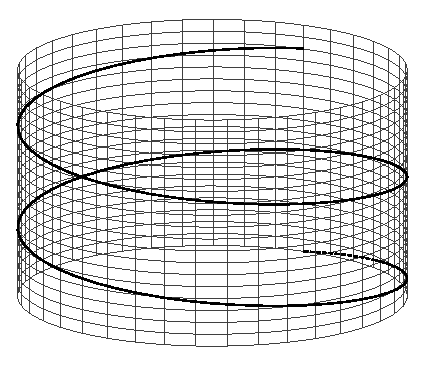
\includegraphics[width=6cm,height=6cm]{figures/cyl}
  \end{center}

  \caption{\small Cylinder surface with a spiral curve.}
  \label{fig-cyl}
\end{figure}

\section{Curves on a cylinder}
We parametrize a curve on the cylinder by letting $\rho,\theta,z$ depend on a single parameter, and thus get the coordinates as a function of $t$.

$$ \vec{r}(t) = (\rho_0\st(t), \rho_0\ct(t), z(t))$$

If we let $\theta(t)=bt$, nd $z(t)=at$, where we can think of $b$ as the rotation speed and $a$ as the speed along the $z$ axis, we obtain

$$ \vec{r}(t) = (\rho_0\sin(bt), \rho_0\cos(bt), at) $$ 
which, with $a=1, b=2$, gives the curve shown in figure \ref{fig-cyl}. The length of this curve is

$$
   l = \int_0^{2\pi}{\sqrt{g_{11}\dot{\theta}^2 + g_{22}\dot{z}^2 }}dt = \int_0^{2\pi}{\sqrt{ b^2\rho_0^2  + a^2 }}dt = 2\pi\sqrt{a^2+b^2\rho_0^2} 
$$

This seems reasonable: When $a=0$ the curve degenerates to a circle with the radius $\rho_0$, and the length is simply the length of the circle, $2\pi\rho_0$, times the number of windings $b$.

\section{Paraboloid}
A well known surface is the \myindx{paraboloid}, which is the same shape as a \myindx{satellite disk}. Its parametrization is
$$
   \vec{r}(u,v) = (u, v, -(u^2 +v^2))
$$

$$
   \vec{e}_1 = \vec{e}_u = \dvd{r}{u} = \left( \begin{array}{c} 
        1 \\
        0 \\
        -2u 
   \end{array} \right)
$$

$$
   \vec{e}_2 = \vec{e}_v = \dvd{r}{v} = \left( \begin{array}{c} 
        0 \\
        1 \\
        -2v 
   \end{array} \right)
$$

\index{metric tensor!paraboloid}
$$
    g_{ij} = \vec{e}_i\cdot\vec{e}_j = \left( \begin{array}{ccc}
      1 +4u^2 & 4uv \\
      4uv & 1 + 4v^2 
    \end{array} \right)
$$
This is the first case where $g_{12}=g_{21}$ is not zero.

\begin{figure}[!ht]
  \begin{center}
    \psset{unit=0.75} 
    \begin{pspicture}(-5.5,-6)(4.5,4) 
      \psset[pst-solides3d]{viewpoint=35 -60 80 rtp2xyz, Decran=50,lightsrc=viewpoint} 
      % Parametric Surfaces
      \defFunction[algebraic]{hyppar}(u,v) 
          {u} {v} {-(u*u + v*v) }
      \defFunction{hypline}(t) 
          {t t Sin mul} {t t Cos mul} { t t mul t Sin t Sin mul t Cos t Cos mul add mul neg }
      \psSolid[object=surfaceparametree, action=draw*, linecolor=black!75,linewidth=0.01, 
          base=pi neg pi pi  neg  pi, fillcolor=blue!20,incolor=black!20, function=hyppar,
          linewidth=0.5 \pslinewidth,ngrid=25]
      \psSolid[object=courbe, r=0, range= pi  neg pi , action=draw*, linecolor=black, 
               linewidth=0.05,resolution=360, function=hypline]
    \end{pspicture}
  \end{center}

  \caption{\small Paraboloid surface.}
  \label{fig-parab}
\end{figure}


\section{Curves on the paraboloid}
The curve on the paraboloid surface shown in figure \ref{fig-parab} is parametrized as
$$
u(t)=t\sin(t),\quad v(t)=t\cos(t), \quad -\pi\le t \le\pi
$$

\begin{align}
   f(t) &= g_{11}\dot{u}^2 +2g_{12}\dot{u}\dot{v}+ g_{22}\dot{v}^2 \notag\\
             &=(1+4t^2\sin^2t)(\sin(t) + t\cos(t))^2\notag\\
             &+ 8t^2\sin(t)\cos(t)(\cos(t) - t\sin(t)) (\sin(t) + t\cos(t))\notag\\
             &+ (1+4t^2\cos^2t)(\cos(t) - t\sin(t))^2 \notag
\end{align}

 and the length of the curve is 

$$
  = \int_{-\pi}^{\pi}{\sqrt{ f(t) }}dt \approx 23.47564\ldots
$$


\section{Hyperbolic paraboloid}
The \myindx{hyperbolic paraboloid} is a surface, shown in figure \ref{fig-hyp_curv}, which can be parametrized by u,v in the following manner
$$
   \vec{r}(u,v) = (u, v, u^2 -v^2)
$$



\begin{figure}[!ht]
  \begin{center}
    \psset{unit=0.75} 
    \begin{pspicture}(-5.5,-6)(4.5,4) 
      \psset[pst-solides3d]{viewpoint=45 210 50 rtp2xyz, Decran=50,lightsrc=45 -50 330} 
      % Parametric Surfaces
      \defFunction[algebraic]{hyppar}(u,v) 
          {u} {v} {(u*u - v*v)/4 }
      \defFunction{hypline}(t) 
          {t t Sin mul} 
          {t t Cos mul} 
          { t t mul t Sin t Sin mul t Cos t Cos mul sub mul 4 div }
      \psSolid[object=surfaceparametree, action=draw*, linecolor=black!75,linewidth=0.01, 
          base=pi neg pi pi  neg  pi, 
          fillcolor=blue!20,incolor=black!20, function=hyppar,linewidth=0.5 \pslinewidth,ngrid=25]
      \psSolid[object=courbe, r=0, range= pi  neg pi , action=draw*, linecolor=black, 
               linewidth=0.05,resolution=360, function=hypline]
    \end{pspicture}
  \end{center}

  \caption{\small Hyperbolic paraboloid surface.}
  \label{fig-hyp_curv}
\end{figure}




$$
   \vec{e}_1 = \vec{e}_u = \dvd{r}{u} = \left( \begin{array}{c} 
        1 \\
        0 \\
        2u 
   \end{array} \right)
$$

$$
   \vec{e}_2 = \vec{e}_v = \dvd{r}{v} = \left( \begin{array}{c} 
        0 \\
        1 \\
        -2v 
   \end{array} \right)
$$

\index{metric tensor!hyperbolic paraboloid}
$$
    g_{ij} = \vec{e}_i\cdot\vec{e}_j = \left( \begin{array}{ccc}
      1 +4u^2 & -4uv \\
      -4uv & 1 + 4v^2 
    \end{array} \right)
$$

The metric tensor is similar to the one for the paraboloid surface, differing only
in the sign of the cross terms.




\section{Curves on the hyperbolic paraboloid}
The curve shown in figure \ref{fig-hyp_curv} is created by the same parametrization as 
for the paraboloid in figure \ref{fig-parab}.
$$
u(t)=t\sin(t),\quad v(t)=t\cos(t),\quad -\pi\le t \le \pi
$$

\begin{align}
   g(t) &= g_{11}\dot{u}^2 +2g_{12}\dot{u}\dot{v}+ g_{22}\dot{v}^2 \notag\\
             &=(1+4t^2\sin^2t)(\sin(t) + t\cos(t))^2\notag\\
             &- 8t^2\sin(t)\cos(t)(\cos(t) - t\sin(t)) (\sin(t) + t\cos(t))\notag\\
             &+ (1+4t^2\cos^2t)(\cos(t) - t\sin(t))^2 \notag
\end{align}

 and the length of the curve is 

$$
  = \int_{-\pi}^{\pi}{\sqrt{ g(t) }}dt \approx 35.57158\ldots
$$


\newcommand{\sh}{a\sin\omega\theta + b} 
\section{Modulated sphere}
A slightly more complicated surface can be created by allowing r to depend on $\theta$ and $\phi$,
For example as $r(\theta,\phi) = \sh$. When $a=0.1, \omega=10, b=1$, the result is the following parametrization of the ``modulated sphere'' shown in figure \ref{fig-def_sph_wind}

\newcommand{\rtp}{r(\theta,\phi)}
$$
  \vec{r}(\theta,\phi) = (\rtp\stsp, \rtp\stcp, \rtp\st)
$$

\begin{figure}[!ht]
  \begin{center}
    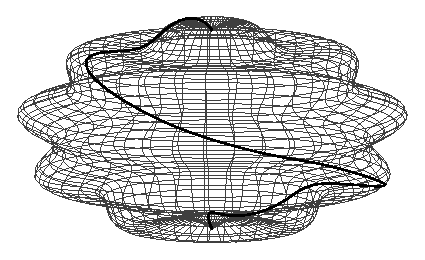
\includegraphics[width=6cm,height=6cm]{figures/def_sph_wind}
  \end{center}

  \caption{\small Modulated sphere ($a=0.1, \omega=10, b=1$)}
  \label{fig-def_sph_wind}
\end{figure}

Now it gets a little complicated..

$$
    \vec{e}_1=\vec{e}_\theta=\dvd{r}{\theta} = 
        \left( \begin{array}{c}
          \left[a\ct\sin(\omega\theta)+a\omega\st\cos(\omega\theta)+b\ct\right] \sip \\ 
          \left[a\ct\sin(\omega\theta)+a\omega\st\cos(\omega\theta)+b\ct\right] \cop \\ 
               -a\st\sin(\omega\theta)+a\omega\ct\cos(\omega\theta)-b\st
        \end{array} \right)
$$

$$
    \vec{e}_2=\vec{e}_\phi=\dvd{r}{\phi} = 
        \left( \begin{array}{c}
         (\sh)\stcp\\ 
         - (\sh)\stsp\\ 
            0
        \end{array} \right)
$$

..and after some manipulations, where we primarily use the \myindx{trigonometric identity} \mbox{$\sin^2a + \cos^2a = 1$}, we get 


$$
    g_{ij} = \vec{e}_i\cdot\vec{e}_j = \left( \begin{array}{ccc}
      f(\theta) & 0 \\
      0  & (\sh)^2\sin^2\theta 
    \end{array} \right)
$$
Where

\begin{align}
 f(\theta) & =   \Big((a\sin(\omega\theta)+b)\ct +a\omega\st\cos(\omega\theta)\Big)^2  \notag\\ 
          & + \Big(-(a\sin(\omega\theta)+b)\st+a\omega\ct\cos(\omega\theta)\Big)^2 \notag\\
          &= (\sh)^2  + a^2\omega^2\cos^2(\omega\theta)\notag 
\end{align}

Note that already at this stage the formulae gets so complicated that there is great risk in not 
getting it right by hand calculation, and no chance of analytic integration. But we can check that 
this is plausible by noting that in the limit of no deformation $(a,b)\to (0,1)$, $f=1$ and we 
recover the metric tensor for the sphere.

\section{Curves on the modulated sphere}
Using the same parametrization, $\theta(t)=t, \phi(t)=2t-\pi$, as for the winding curve on the sphere we get a complicated curve as shown in figure \ref{fig-def_sph_wind}. Since
$$
   g_{11}\dot{\theta}^2 + g_{22}\dot{\phi}^2 = f(t) + 4(a\sin\omega t + b)^2\sin^2t
$$
we obtain the formula for the curve length as 

$$
   l = \int_0^\pi{\sqrt{ f(t) + 4(a\sin\omega t + b)^2\sin^2t }}dt \approx 5.73653\ldots
$$





  \chapter{Curvature}

In this chapter we will give the formulae for working with
curvatures. This part is filled with symbols which makes it somewhat hard
to comprehend. Just consider the symbols as functions which can be
calculated from the metric tensor. 

\index{curvature!Gaussian}
\section{\myindx{Gaussian Curvature}}
Gauss' curvature formula describes the curvature of a two dimensional
surface parametrized by $(u,v)$.


$$
K = -\frac{1}{g_{11}} \left( \frac{\partial}{\partial u}\Gamma_{12}^2 - \frac{\partial}{\partial v}\Gamma_{11}^2 + \Gamma_{12}^1\Gamma_{11}^2 - \Gamma_{11}^1\Gamma_{12}^2 + \Gamma_{12}^2\Gamma_{12}^2 - \Gamma_{11}^2\Gamma_{22}^2\right)
$$

\section{Riemann curvature tensor}
\index{Riemann tensor} 
\index{curvature!Riemann}

The Riemann curvature tensor is a tensor of the fourth order, which 
is defined in the following way
$$
{R^\rho}_{\sigma\mu\nu} = \partial_\mu\Gamma^\rho_{\nu\sigma}
    - \partial_\nu\Gamma^\rho_{\mu\sigma}
    + \Gamma^\rho_{\mu\lambda}\Gamma^\lambda_{\nu\sigma}
    - \Gamma^\rho_{\nu\lambda}\Gamma^\lambda_{\mu\sigma}
$$

\section{Ricci curvature tensor}
\index{curvature!Ricci}
The \myindx{Ricci tensor} is related to the Riemann curvature 
tensor by contracting two indices
$$
   R_{\sigma\nu} = {R^\rho}_{\sigma\rho\nu} =
{\Gamma^\rho_{\nu\sigma}}_{,\rho} - \Gamma^\rho_{\rho\sigma ,\nu}
+ \Gamma^\rho_{\rho\lambda} \Gamma^\lambda_{\nu\sigma}
- \Gamma^\rho_{\nu\lambda}\Gamma^\lambda_{\rho\sigma}
$$


\myhrule
\begin{myex}
For the spherical surface with unit length the only nonzero Christoffel
symbols are
\begin{eqnarray*}
   \Gamma^2_{12} &=& \;\;\frac{\cos\theta}{\sin\theta} \\
   \Gamma^1_{22} &=& -\cos\theta\sin\theta
\end{eqnarray*}
of which only $\Gamma^2_{12}$ appears in Gauss' formula.
Noting that $g_{11}=1$, the Gaussian curvature is then

$$
    K = -\frac{d}{d\theta}\frac{\cos\theta}{\sin\theta} - \left( \frac{\cos\theta}{\sin\theta} \right)^2 = 1
$$
which shows that the sphere has a constant, positive curvature.
\end{myex}


\begin{myex}
A for the hyperbolic paraboloid, the  nonzero Christoffel symbols are
\begin{eqnarray*}
   \Gamma_{11}^1 &=&  \;\;\frac{4u}{4v^2+4u^2+1} \\ 
   \Gamma_{11}^2 &=& -\frac{4v}{4v^2+4u^2+1} \\ 
   \Gamma_{22}^1 &=& -\frac{4v}{4v^2+4u^2+1} \\ 
   \Gamma_{22}^2 &=& \;\;\frac{4v}{4v^2+4u^2+1} 
\end{eqnarray*}
the gaussian formula reduces to
$$
   K = \frac{1}{g_{11}} \left(\frac{d}{dv}\Gamma_{11}^2 + \Gamma_{11}^2\Gamma_{22}^2 \right)
     = -\frac{4}{(4v^2+4u^2+1)^2}
$$
The Gaussian curvature is now a function of $u$, and $v$,
and we see that this surface has negative curvature everywhere with a minimum
occuring at $(u,v)=(0,0)$, where it has the value $-4$.
\end{myex}


  \newcommand{\lcs}{\Gamma}
\newcommand{\mcs}[2]{\Gamma_{#1}^{#2}}

\chapter{Tensor Examples}
\label{sec:christoffel}

In this section we will give some examples of the Christoffel symbols (of 
both kinds) derived from specific coordinate systems. It will be demonstrated
that depending on the metric tensor components there can be few or many of either 
kind. 

When working with tensors and their \myindx{derivatives}, such as the ones 
needed for calculating the \myindx{Christoffel symbols}, it is very time 
consuming to do these calculations by hand. 
To demonstrate the complexity of this \myindx{algebraic manipulation} let us 
calculate $\Gamma^2_{12}$ for the \myindx{spherical coordinates} described in section \ref{sec:sphcoord}.

$$
    \Gamma^2_{12} = \frac{1}{2} g^{2m} \left( \frac{\partial g_{m1}}{\partial u^2}  
                 +\frac{\partial g_{m2}}{\partial u^1}
                 -\frac{\partial g_{12}}{\partial u^m}
       \right)
$$

since $u^1=r, u^2=\theta$, and $u^3=\phi$ we get, when summing over $m=1,2,3$

$$
  \begin{array}{llllll}
    \Gamma^2_{12}  &= &\frac{1}{2} g^{21} \left( \frac{\partial g_{11}}{\partial \theta}  
                 +\frac{\partial g_{12}}{\partial r}
                 -\frac{\partial g_{12}}{\partial r} \right) +
                 \frac{1}{2} g^{22} \left( \frac{\partial g_{21}}{\partial \theta}  
                 +\frac{\partial g_{22}}{\partial r}
                 -\frac{\partial g_{12}}{\partial \theta} \right) \\ 
             &&+ 
                 \frac{1}{2} g^{23} \left( \frac{\partial g_{31}}{\partial \theta}  
                 +\frac{\partial g_{32}}{\partial r}
                 -\frac{\partial g_{12}}{\partial \phi} \right) \\
          & = &\frac{1}{2} g^{22}\frac{\partial g_{22}}{\partial r} = \frac{1}{2}\frac{1}{r^2}(2r) = \frac{1}{r}
  \end{array}
$$
It turns out that all but one derivative of the metric tensor are zero, but this is not
always the case! Note that there are $N^3$ Christoffel symbols, so in three dimensions we need to 
do this 27 times performing $9*27=243$ derivatives!

Clearly the possibility for errors is significant, so why not let a symbolic math program handle the 
tiresome and error prone calculations? After all this has been done by professionals 
since 1966 \cite{misner}.  The following examples were created using 
\myindx{Maxima} \cite{maxima}. For source code examples see 
section \ref{sec:maxima}.

The Christoffel symbol of the first kind is defined as 

$$
    \Gamma_{ijk} = \frac{1}{2} \left( \frac{\partial g_{ik}}{\partial u^j}  
                 +\frac{\partial g_{jk}}{\partial u^i}
                 -\frac{\partial g_{ij}}{\partial u^k}
       \right)
$$
and the Christoffel symbol of the second kind is 
$$
    \Gamma^k_{ij} = \frac{1}{2} g^{km} \left( \frac{\partial g_{mi}}{\partial u^j}  
                 +\frac{\partial g_{mj}}{\partial u^i}
                 -\frac{\partial g_{ij}}{\partial u^m}
       \right)
$$


In the following we will calculate the Christoffel symbols of the first and second kind for 
a number of coordinate systems using these formulae.


\section{Cylindrical Coordinates}

From section \ref{sec:cylcoord} we have

$$
   \vec{r}(\rho,\phi,z) = (\rho \cos(\phi), \rho \sin(\phi), z)
$$

and 



\begin{eqnarray*}
\lcs_{122}=&\rho, \qquad \lcs_{221}=&-\rho
\end{eqnarray*}

$$
g^{ij} = \begin{pmatrix}
   1 &      0          & 0\cr 
   0 &\frac{1}{\rho^2} & 0\cr 
   0 &      0          & 1\cr 
\end{pmatrix}
$$

\begin{eqnarray*}
\mcs{12}{2}=&\frac{1}{\rho}, \qquad \mcs{22}{1}=&-\rho
\end{eqnarray*}


\section{\myindx{Spherical Coordinates}}
\label{sec:maxima_sph}

Of the 27 potential Christoffel symbols of the first kind, only six are 
nonzero and only three needs to be calculated due to symmetry properties.

\begin{twocol}{
\begin{eqnarray*}
\lcs_{122}=&r \\
\lcs_{133}=&r\,\cos ^2\theta \\
\lcs_{221}=&-r \\
\end{eqnarray*}}{
\begin{eqnarray*}
\lcs_{233}=&-r^2\,\cos \theta\,\sin \theta \\
\lcs_{331}=&-r\,\cos ^2\theta \\
\lcs_{332}=&r^2\,\cos \theta\,\sin \theta
\end{eqnarray*}}
\end{twocol}

The inverse of $g_{ij}$ is

$$ 
    g^{ij}=\begin{pmatrix}1&0&0\cr 0&\frac{1}{r^2}&0\cr 0&0&\frac{1}{r^2\,\cos ^2
 \theta}\cr \end{pmatrix}
$$


From this we can calculate the Christoffel symbols of second kind. 

\begin{twocol}{
\begin{eqnarray*}
\mcs{12}{2}=&\frac{1}{r} \\
\mcs{13}{3}=&\frac{1}{r} \\
\mcs{22}{1}=&-r \\
\end{eqnarray*}}{
\begin{eqnarray*}
\mcs{23}{3}=&-\frac{\sin \theta}{\cos \theta} \\
\mcs{33}{1}=&-r\,\cos ^2\theta \\
\mcs{33}{2}=&\cos \theta\,\sin \theta \\
\end{eqnarray*}}
\end{twocol}{


\section{Ellipsoidal Coordinates}
If we take the innocent spherical coordinates and change them in the following way

$$
   \vec{r}(u,v,w) = (a u \sin v \cos w, bu\sin v \sin w, c u \cos v)
$$
we get the \myindx{ellipsoidal coordinates}
where $r$ has been replaced by $u$, $\theta$ by $v$ and $\phi$ by $w$ we get for the 
metric tensor $g_{ij}=$


\begin{wide}
$$
   \begin{pmatrix}

  \sin^2v(b^2\sin ^2w+a^2\cos ^2w)+c^2\cos ^2v   &
  u\cos v \sin v(b^2\sin ^2w+a^2\cos ^2 w-c^2)  &
  \left(b^2-a^2\right)u\sin ^2v\cos w \sin w\cr 

  u\cos v \sin v(b^2\sin ^2w+a^2 \cos ^2w-c^2)  &
  u^2\cos^2v(b^2\sin ^2w+a^2\cos ^2w)+c^2u^2\sin ^2v  &
  \left(b^2-a^2\right)u^2 \cos v\sin v\cos w\sin w\cr 

  \left(b^2-a^2\right)u\sin ^2v \cos w\sin w   &
  \left(b^2-a^2\right)u^2\cos v\sin v\cos w \sin w   &
   a^2u^2\sin ^2v\sin ^2w+b^2u^2\sin ^2v\cos ^2w\cr 
   \end{pmatrix}
$$
\end{wide}
... and as you can see the page is barely wide enough to hold the result even with a tiny font!  But from
Maxima we get the following 15 Christoffel symbols of the first kind

\begin{eqnarray*}
\Gamma_{121}=&\cos v\,\sin v\,\left(b^2\,\sin ^2w+a^2\,\cos ^2w
 -c^2\right)\\
\Gamma_{122}=&u\,\left(b^2\,\cos ^2v\,\sin ^2w+a^2\,\cos ^2v\,
 \cos ^2w+c^2\,\sin ^2v\right)\\
\Gamma_{123}=&\left(b-a\right)\,\left(b+a\right)\,u\,\cos v\,
 \sin v\,\cos w\,\sin w\\
\Gamma_{131}=&\left(b-a\right)\,\left(b+a\right)\,\sin ^2v\,
 \cos w\,\sin w\\
\Gamma_{132}=&\left(b-a\right)\,\left(b+a\right)\,u\,\cos v\,
 \sin v\,\cos w\,\sin w\\
\Gamma_{133}=&u\,\sin ^2v\,\left(a^2\,\sin ^2w+b^2\,\cos ^2w
 \right)\\
\Gamma_{221}=&-u\,\left(b^2\,\sin ^2v\,\sin ^2w+a^2\,\sin ^2v\,
 \cos ^2w+c^2\,\cos ^2v\right)\\
\Gamma_{222}=&-u^2\,\cos v\,\sin v\,\left(b^2\,\sin ^2w+a^2\,
 \cos ^2w-c^2\right)\\
\Gamma_{223}=&-\left(b-a\right)\,\left(b+a\right)\,u^2\,\sin ^2
 v\,\cos w\,\sin w\\
\Gamma_{231}=&\left(b-a\right)\,\left(b+a\right)\,u\,\cos v\,
 \sin v\,\cos w\,\sin w\\
\Gamma_{232}=&\left(b-a\right)\,\left(b+a\right)\,u^2\,\cos ^2v
 \,\cos w\,\sin w\\
\Gamma_{233}=&u^2\,\cos v\,\sin v\,\left(a^2\,\sin ^2w+b^2\,
 \cos ^2w\right)\\
\Gamma_{331}=&-u\,\sin ^2v\,\left(b^2\,\sin ^2w+a^2\,\cos ^2w
 \right)\\
\Gamma_{332}=&-u^2\,\cos v\,\sin v\,\left(b^2\,\sin ^2w+a^2\,
 \cos ^2w\right)\\
\Gamma_{333}=&-\left(b-a\right)\,\left(b+a\right)\,u^2\,\sin ^2
 v\,\cos w\,\sin w\\
\end{eqnarray*}

You can verify that this seems reasonable by setting $a=b=c=1$ in which case many of these
become zero and we are left with the six symbols from the Spherical coordinates. The formula
for the inverse of the metric tensor is not given as it turns out to be quite big, but using
Maxima we can calculate the Christoffel symbols of the second kind and there turns out to be six
of these just as in the case of the Spherical coordinates.

\begin{twocol}{
\begin{eqnarray*}
\Gamma_{12}^{2}=&{{1}\over{u}}\\
\Gamma_{13}^{3}=&{{1}\over{u}}\\
\Gamma_{22}^{1}=&-u\\
\end{eqnarray*}}{
\begin{eqnarray*}
\Gamma_{23}^{3}=&{{\cos v}\over{\sin v}}\\
\Gamma_{33}^{1}=&-u\,\sin ^2v\\
\Gamma_{33}^{2}=&-\cos v\,\sin v\\
\end{eqnarray*}}
\end{twocol}


\section{Other Coordinates}
This coordinate system is taken from \cite{night} p. 11. It 
probably does not have any practical applications, but it is the first
example of a metric tensor where all components are nonzero.

$$
    \vec{r}(u,v,w) = (u+v, u-v, 2uv + w)
$$

$$
   g_{ij} = \begin{pmatrix}
               4v^2 +2 & 4uv & 2v \\
               4uv & 4u^2 + 2 & 2u \\
               2v & 2u & 1
            \end{pmatrix}
$$

There are only three Christoffel symbols of the first kind
\begin{eqnarray*}
\lcs_{121}=&4v \\
\lcs_{122}=&4u \\
\lcs_{123}=&2
\end{eqnarray*}

The inverse of the metric tensor is

$$
   g^{ij} = \begin{pmatrix}
               1/2  & 0  & -v \\
               0 & 1/2 & -u  \\
               -v & -u & 2v^2 + 2u^2+1 
            \end{pmatrix}
$$
This means that we are left with only one Christoffel symbol of the second kind
\begin{eqnarray*}
\mcs{12}{3}=&2 \\
\end{eqnarray*}

\section{\myindx{Geodesics}}

Why bother with all these Christoffel symbols? The reason is that in order to find
the \myindx{equations of motions} in General Relativity we need to find the possible 
patterns of movements (straight lines) and these are called Geodesics. There is a connection between
Geodesics and the Christoffel symbols given by 

$$
    \frac{d^2u^i}{dt^2} + \Gamma_{jk}^i\frac{du^j}{dt}\frac{du^k}{dt} = 0
$$

Now let us take the Spherical coordinate system and find the Geodesic curves. First by
noting that $u^i=u^1=r$,

\begin{eqnarray}
    \frac{d^2r}{dt^2} + \Gamma_{jk}^1\frac{du^j}{dt}\frac{du^k}{dt} = 0 \\
    \frac{d^2r}{dt^2} + \Gamma_{22}^1(\dot{\theta})^2
    + \Gamma_{33}^1(\dot{\phi})^2 = 0
\end{eqnarray}
here $u^i=u^2=\theta$,
$$
    \frac{d^2\theta}{dt^2} + \Gamma_{jk}^2\frac{du^j}{dt}\frac{du^k}{dt} = 0
$$
$$
    \frac{d^2\theta}{dt^2} + \Gamma_{12}^2\dot{r}\dot{\theta}
    + \Gamma_{33}^2(\dot{\phi})^2 = 0
$$

finally by setting $u^i=u^3=\phi$, we get
\begin{eqnarray*} 
    \frac{d^2\phi}{dt^2} + \Gamma_{jk}^3\frac{du^j}{dt}\frac{du^k}{dt} = 0 \\
    \frac{d^2\phi}{dt^2} + \Gamma_{13}^3\dot{r}\dot{\phi}
    + \Gamma_{23}^3\dot{\theta}\dot{\phi} = 0
\end{eqnarray*}
so the equations of motion are given by the three second-order differential
equations
\begin{eqnarray*} 
    \ddot{r} -r\dot{\theta}^2 -r \cos^2\theta\dot{\phi}^2 = 0\\
    \ddot{\theta} + \frac{1}{r}\dot{r}\dot{\theta}
    + \cos\theta\sin\theta(\dot{\phi})^2 = 0 \\
    \ddot{\phi} + \frac{1}{r}\dot{r}\dot{\phi}
    - \frac{sin\theta}{\cos\theta}\dot{\theta}\dot{\phi} = 0
\end{eqnarray*}
This seems complicated, but let us see what it means in a simple case, where $\theta$ is 
constant at $\theta_0$ and $r=1$. In this case the equations reduce to

\begin{eqnarray}
    -cos^2\theta_0\dot{\phi}^2 = 0\\
    \ddot{\phi}  = 0
\end{eqnarray}

from the first equation we get $\theta_0=\pi/2$, and from the second equation we get
$\phi(t) = at+b$.

This means that the geodesic curves of constant $\theta$ and $r$ are great circles on the 
equator.

\fixme{Find a better (simpler) example?}

\section{Higher dimensional spaces}
\subsection{\myindx{Schwarzchild metric (4d)}}
\label{sec:schwarz}
An important metric in General Relativity is the Schwarzchild metric which is a topic in 
section \ref{sec:4dcurves}. When the four coordinates are $t, r, \theta, \phi$, and 
 $a=GM/c^2$ and spherical coordinates are used, its metric tensor is

$$
g_{ij}= 
\begin{pmatrix}
1-{{a}\over{r}}&0&0&0\cr 
0&-{{1}\over{1-{{a}\over{r}}}}&0& 0\cr 
0&0&-r^2&0\cr 0&0&0&-r^2\sin ^2\theta\cr 
\end{pmatrix}
$$

The Christoffel symbols of the first kind are

\begin{twocol}{
\begin{eqnarray*}
\Gamma_{112}=&{{ar-a^2}\over{2r^3}}\\
\Gamma_{121}=&{{a}\over{2r^2-2ar}}\\
\Gamma_{222}=&-{{a}\over{2r^2-2ar}}\\
\Gamma_{233}=&{{1}\over{r}}\\
\Gamma_{244}=&{{1}\over{r}}\\
\end{eqnarray*}
}{
\begin{eqnarray*}
\Gamma_{332}=&a-r\\
\Gamma_{344}=&{{\cos \theta}\over{\sin \theta}}\\
\Gamma_{442}=&\left(a-r\right)\sin ^2\theta\\
\Gamma_{443}=&-\cos \theta\sin \theta\\
\end{eqnarray*}
}
\end{twocol}

and the inverse metric tensor is 
$$
g^{ij} = 
\begin{pmatrix}
{{1}\over{1-{{a}\over{r}}}}&0&0&0\cr 0&{{a}\over{r}}-1&0&0
 \cr 0&0&-{{1}\over{r^2}}&0\cr 0&0&0&-{{1}\over{r^2\sin ^2\theta
 }}\cr 
\end{pmatrix}
$$

and the Christoffel symbols of the second kind are given as 

\begin{twocol}{
\begin{eqnarray*}
\Gamma_{11}^{2}=&-{{a}\over{2r^2}}\\
\Gamma_{12}^{1}=&{{a}\over{2r^2}}\\
\Gamma_{22}^{2}=&{{a}\over{2\left(1-{{a}\over{r}}\right)^2r^2 }}\\
\Gamma_{23}^{3}=&-r\\
\end{eqnarray*}}
{
\begin{eqnarray*}
\Gamma_{24}^{4}=&-r\sin ^2\theta\\
\Gamma_{33}^{2}=&r\\
\Gamma_{34}^{4}=&-r^2\cos \theta\sin \theta\\
\Gamma_{44}^{2}=&r\sin ^2\theta\\
\Gamma_{44}^{3}=&r^2\cos \theta\sin \theta\\
\end{eqnarray*}}
\end{twocol}

\subsection{\myindx{Kaluza-Klein metric (5d)}}
A space of five dimensions were contrieved in a unification theory by Kaluza and Klein.
Several variations of the theme exist, but the following is an example from \cite{art:tiwari} where
the  metric tensor is


$$
 \hat{g}_{\hat{\mu}\hat{\nu}} = 
     \begin{pmatrix}
         1  &  0  &  0   &  0                 & 0 \\
         0  & -A^2(t)  &  0   &  0                 & 0 \\
         0  &  0  & -A^2(t)r^2 &  0                 & 0 \\
         0  &  0  &  0   & -A^2(t)r^2\sin^2\theta & 0 \\
         0  &  0  &  0   &  0                 & -B^2(t) 
    \end{pmatrix} 
$$
the inverse of the metric tensor is 
$$
 \hat{g}^{\hat{\mu}\hat{\nu}} = 
     \begin{pmatrix}
         1  &  0  &  0   &  0                 & 0 \\
         0  & -\frac{1}{A^2(t)}  &  0   &  0                 & 0 \\
         0  &  0  & -\frac{1}{A^2(t)r^2} &  0                 & 0 \\
         0  &  0  &  0   & -\frac{1}{A^2(t)r^2\sin^2\theta} & 0 \\
         0  &  0  &  0   &  0                 & -\frac{1}{B^2(t)} 
    \end{pmatrix} 
$$
and the Christoffel symbols of the second kind are



\begin{twocol}{
\begin{eqnarray*}
\Gamma_{12}^{2}=&\frac{\dot{A}}{A}\\
\Gamma_{13}^{3}=&\frac{\dot{A}}{A}\\
\Gamma_{14}^{4}=&\frac{\dot{A}}{A}\\
\Gamma_{15}^{5}=&\frac{\dot{B}}{B}\\
\Gamma_{22}^{1}=&A\dot{A}\\
\Gamma_{23}^{3}=&\frac{1}{r}\\
\Gamma_{24}^{4}=&\frac{1}{r}
\end{eqnarray*}
}{
\begin{eqnarray*}
\Gamma_{33}^{1}=&r^2A\dot{A}\\
\Gamma_{33}^{2}=&-r\\
\Gamma_{34}^{4}=&\frac{\cos\theta}{\sin\theta}\\
\Gamma_{44}^{1}=&r^2\sin^2\theta A\dot{A}\\
\Gamma_{44}^{2}=&-r\sin^2\theta\\
\Gamma_{44}^{3}=&-\cos\theta\sin\theta\\
\Gamma_{55}^{1}=&B\dot{B}
\end{eqnarray*}}
\end{twocol}
which is not too bad considering that there could have been $5^3=125$!. Note that the symbols depend 
on the choice of the functions $A(t)$ and $B(t)$ and their
derivatives. The functions would have to be found as a solution to the Einstein field equations,
but one could assume a form of the functions and then calculate the consequences for 
\myindx{cosmology}.


  \newcommand{\ia}{0.6} % Theta_zero
\newcommand{\ib}{0.0} % Angle from due south (alpha in foster et al. p. 68)

\chapter{Parallel Transport}
\label{sec:parallel}
\index{parallel transport}

In this chapter we will discuss parallel transport of vectors along a curve. This turns out
to be an important concept because it is closely related to Geodesics and the possible
solutions to the equations of motion in spacetime. We will start by going through an example
from \cite{night} to illustrate the ideas. We wish to make a parallel transport of a vector 
pointing 'south' along a curve of constant latitude $\theta_0$. 

\begin{figure}[!ht]
\begin{center}
  \begin{pspicture}(-4,-4)(4,4)
    \psset{unit=3cm}
    \parametricplotThreeD[linewidth=0.5pt, plotstyle=curve,yPlotpoints=20](0,360)(0,360)
        {t cos u sin mul t cos u cos mul t sin} 

    \parametricplotThreeD[linewidth=0.5pt,plotstyle=curve,yPlotpoints=20](0,360)(0,360)
        {u cos t sin mul u cos t cos mul u sin}

    \pstThreeDSphere[SegmentColor={[cmyk]{0,0,0,0}}](0,0,0){1} 

    \pstThreeDCoor[linewidth=1.0pt,xMin=-1.5,xMax=1.5, yMax=1.5, zMax=1.5] 

    \parametricplotThreeD[algebraic,plotstyle=curve,linewidth=1.5pt](0,3.1415 2 mul)
          {sin(\ia)*cos(t)| sin(\ia)*sin(t)|cos(\ia)}

    \multido{\rtt=0.0+0.3141592}{21}{
      \parametricplotThreeD[algebraic,plotstyle=curve,linewidth=1.0pt, linecolor=blue, arrows=->](0.0,0.3 )
          { sin(\ia)*cos(\rtt)+( cos(\ia)*cos(\rtt)*cos( \ib - cos(\ia)*\rtt ) - sin(\rtt)*sin(\ib - cos(\ia)*\rtt) )*t 
          | sin(\ia)*sin(\rtt)+( cos(\ia)*sin(\rtt)*cos( \ib - cos(\ia)*\rtt ) + cos(\rtt)*sin(\ib - cos(\ia)*\rtt) )*t
          | cos(\ia)          +(-sin(\ia)          *cos( \ib - cos(\ia)*\rtt ) + 0                                  )*t }
       }
%    \renewcommand{\ia}{1.57}
%    \multido{\rtq=0.0+0.3141592}{21}{
%      \parametricplotThreeD[algebraic,plotstyle=curve,linewidth=1.0pt, linecolor=blue, arrows=->](0.0,0.3 )
%          { sin(\ia)*cos(\rtq)+( cos(\ia)*cos(\rtq)*cos( \ib - cos(\ia)*\rtq ) - sin(\rtq)*sin(\ib - cos(\ia)*\rtq) )*t 
%          | sin(\ia)*sin(\rtq)+( cos(\ia)*sin(\rtq)*cos( \ib - cos(\ia)*\rtq ) + cos(\rtq)*sin(\ib - cos(\ia)*\rtq) )*t
%          | cos(\ia)          +(-sin(\ia)          *cos( \ib - cos(\ia)*\rtq ) + 0                                  )*t }
%       }

  \end{pspicture}
  \caption{\small Parallel transport of a vector around a circle at constant latitude $\theta_0$ on 
           the surface of a sphere, following the example in \cite{night} p. 68. Here
           $\alpha=0, \theta_0=0.6$.}
  \label{fig-parallel}
\end{center}
\end{figure}

\newcommand{\laet}{\lambda^1}
\newcommand{\lato}{\lambda^2}

$$
   \lambda = \laet \eet + \lato \eto
$$
where ...
$$
   \vec{v} = \vec{r}(r_0, \theta, \phi) + \left[ \laet \eet + \lato \eto \right]t
$$
setting $r=1$, we get a parametric representation of the 
transported vector  as a function of t for a given position on the sphere $(\theta, \phi)$.

For transport on a circle at latitude $\theta_0$
$$
v(t)_{\theta,\phi}= \begin{pmatrix}
                      \stcp \\
                      \stsp \\
                      \ct 
                    \end{pmatrix}
   + \left[ \cos(\alpha -\phi\ct) \begin{pmatrix}
                      \ctcp \\
                      \ctsp \\
                      -\st 
                    \end{pmatrix}
   +  \frac{\sin(\alpha-\phi\ct)}{\sin\theta} \begin{pmatrix}
                      -\stsp \\
                      \stcp \\
                      0 
                    \end{pmatrix}
      \right] t
$$


  \chapter{Curves in higher dimensions}
\label{sec:4dcurves}

There is no reason to stop at 3D as mathematics do not
place any limits on curves.

In fact General Relativity operates with the notion of \myindx{spacetime} which 
is a four dimensional construction, and in other areas of physics
even higher dimensions are used. \myindx{String theory} which tries to 
unite the four fundmental forces operates with dimensions of 10 and
upwards. Moving to higher dimensions, however, presents some difficulties as 
1) the metric tensor has higher dimensionality and hence more terms and 
cross terms to evaluate. 2) For dimensions higher than 3 graphical visualization
is impossible.


\section{Spacetime}
Spacetime is the incorporation of time as a fourth coordinate into three dimensional space.
$$
    u_\nu = (x_0, x_1, x_2, x_3) = (ct, -x, -y, -z)
$$
With the metric tensor
\index{metric tensor!spacetime}
$$
   g_{\mu\nu} = \begin{pmatrix}
       c &  0 &  0 &  0 \\ 
       0 & -1 &  0 &  0 \\ 
       0 &  0 & -1 &  0 \\ 
       0 &  0 &  0 & -1 \\ 
   \end{pmatrix} 
$$
and a the distance between nearby points is $\Delta s^2 = c^2dt^2 - dx^2 - dy^2 - dz^2$.

Note that since all elements of $g$ are constant, all Christoffel symbols are $0$, this space
is flat!


\section{\myindx{Schwarzchild Metric}}
The Schwarzchild metric is a specific solution to Einsteins field equations for gravitation
around a massive object in empty space given spherical symmetry. Examples of the derivation
of this metric are given in \cite{night} and \cite{padman}.

\index{metric tensor!Schwarzchild}
$$
   g_{\mu\nu} = \begin{pmatrix}
        1 - 2MG/c^2r & 0                  &   0  & 0     \\
        0            & -(1-2MG/c^2r)^{-1} &   0  & 0     \\
        0            &                    & -r^2 & 0     \\
        0            &         0          &   0  & -r^2\sin^2\theta 
      \end{pmatrix}
$$
the Christoffel symbols for this metric are given in section \ref{sec:schwarz}.


\begin{figure}
\begin{center}
\psset{unit=0.75} 
\begin{pspicture}(-5.5,-7)(4.5,4) 
  \psset[pst-solides3d]{viewpoint=20 120 30 rtp2xyz, Decran=50,lightsrc=10 125 20 rtp2xyz}
  % Parametric Surfaces
  \defFunction{hole}(u,v) 
      {u} 
      {v} 
      { 1 neg u dup mul v dup mul add 0.2 add div}
  \defFunction{curve}(t) 
      {t Cos 3 mul 1.5 sub} 
      {t Sin 3 mul 1.5 add} 
%      { 0}
      { 1 neg t Cos 3 mul 1.5 sub dup mul t Sin 3 mul 1.5 add dup mul add 0.2 add div}
  \psSolid[object=surfaceparametree, linecolor=black!70, base=3 neg 3 3 neg 3, 
         fillcolor=blue!50,incolor=black!90, function=hole,linewidth=0.5\pslinewidth,ngrid =30]% 
      \psSolid[object=courbe, r=0, range= 0.5 2.05 neg , action=draw*, linecolor=black, 
               linewidth=0.05,resolution=360, function=curve]
\end{pspicture}
\end{center}
\vspace{1cm}
\begin{center}
 \caption{\small Curvature of space near a massive object.}
\end{center}
\end{figure}


\section{\myindx{Kerr Metric}}
For a rotating massive object the metric tensor is a further generalization of the Schwarzchild 
metrix, where

\index{metric tensor!Kerr}
$$
   g_{\mu\nu} = \begin{pmatrix}
      \left( 1 - \frac{r_sr}{\rho^2}c^2 \right) & 0 & 0 & \frac{r_sr\alpha\sin^2\theta}{\rho^2} \\
      0         & - \frac{\rho^2}{\Delta} & 0 &  0 \\
      0 & 0 & -\rho^2 & 0 \\ 
      \frac{r_sr\alpha\sin^2\theta}{\rho^2} & 0 & 0 & \left( r^2 + \alpha^2 + \frac{r_sr\alpha^2}{\rho^2}\sin^2\theta\right)\sin^2\theta 
      \end{pmatrix}
$$
where 

\begin{twocol}{
\begin{eqnarray*}
   r_s =& \frac{2GM}{c^2} \\
   \alpha =& \frac{J}{Mc} \\
\end{eqnarray*}}{
\begin{eqnarray*}
   \rho^2 =& r^2 + \alpha^2\cos^2\theta \\
   \Delta =& r^2 -r_sr + \alpha^2 
\end{eqnarray*}}
\end{twocol}

In the limit of no rotation (where $J=0$) the metric reduces to the Schwarzchild metric.

\section{\myindx{Robertson-Walker Metric}}
\myindx{Friedmann}
\myindx{Lema\^itre}
\myindx{Einstein field equations}

Or Friedmann-Lema\^itre-Robertson-Walker metric as it probably should be named due to its 
many contributors.  This is another exact solution of the Einstein Field equations in the context 
\myindx{cosmology}, where a homogenous and isotropic, expanding (or contracting) universe is 
described. The metric tensor is given as 

\index{metric tensor!Robertson-Walker}
$$
 g_{\mu\nu} =   \begin{pmatrix}
    c^2 & 0 & 0 & 0 \\
    0 & -A(t)^2\frac{1}{1-kr^2} & 0 & 0 \\
    0 & 0 & -A(t)^2r^2 & 0 \\
    0 & 0 &  0 & -A(t)^2r^2\sin^2\theta
    \end{pmatrix}
$$
where $A(t)$ is a \myindx{scale factor} affecting the spatial components.

$$
 g^{\mu\nu} =   \begin{pmatrix}
   \frac{1}{c^2} & 0 & 0 & 0\\
   0 & -\frac{1+kr^2}{A^2} & 0 & 0 \\
   0 & 0 & -\frac{1}{r^2A^2} & 0 \\
   0 & 0 & 0 & -\frac{1}{A^2r^2\sin^2\theta} 
  \end{pmatrix}
$$
and 

\begin{twocol}{
\begin{eqnarray*}
   \Gamma_{12}^2 = \frac{\dot{A}}{A} \\
   \Gamma_{13}^3 = \frac{\dot{A}}{A} \\
   \Gamma_{14}^4 = \frac{\dot{A}}{A} \\
   \Gamma_{22}^1 = \frac{A\dot{A}}{c^2(1+kr^2)} \\
   \Gamma_{22}^2 = -\frac{kr}{1+kr^2} \\
   \Gamma_{23}^3 = \frac{1}{r} \\
\end{eqnarray*}}{
\begin{eqnarray*}
   \Gamma_{24}^4 = \frac{1}{r} \\
   \Gamma_{33}^1 = \frac{r^2A\dot{A}}{c^2} \\
   \Gamma_{33}^2 = -r(1+kr^2) \\
   \Gamma_{34}^4 = \frac{\cos\theta}{\sin\theta} \\
   \Gamma_{44}^1 = \frac{r^2A\dot{A}\sin^2\theta}{c^2} \\
\end{eqnarray*}}
\end{twocol}


  \appendix
  
\chapter{Notation and Symbols}

{\renewcommand{\tabcolsep}{0.2cm}
\renewcommand{\arraystretch}{1.3}
\begin{tabular}{|l|l|}
\hline
\textbf{Notation} & \textbf{Meaning} \\
\hline

$a$  & The scalar $a$  \\
\hline

$\vp$  & The vector $\vp$  \\
\hline

$\vec{e}_i$  & Basis vectors in any coordinate system, i=1...N  \\
\hline

$u^i$  & Coordinates in any coordinate system, i=1...N  \\
\hline

$|\vp|$  & Length of vector $\vp$  \\
\hline

$\dot{f}$ & Differentiation of $f$ with respect to time $t$\\
\hline

$\ddot{f}$ & Second order differentiation of $f$ with respect to time $t$\\
\hline

$\vp \cdot \vq$  & Dot product of vectors $\vp$ and $\vq$  \\
\hline

$\vp\times \vq$  & Cross product of vectors $\vp$ and $\vq$ \\
\hline

$g_{ij}$  & Components of the metric tensor\\
\hline

$g^{ij}$  & Components of the inverse of the metric tensor\\
\hline

$\Gamma_{ijk}$  & Christoffel symbol of the first kind\\
\hline

$\Gamma^k_{ij}$  & Christoffel symbol of the second kind\\
\hline

$R_{ij}$  & Ricci tensor\\
\hline

$R_{ijkl}$  & Riemann tensor\\
\hline

$R_{jkl}^i$  & Riemann tensor\\
\hline

\end{tabular}
}

  \newcommand{\mypeople}[4]{
\index{#1}
\noindent{ \textbf{#1} (#2):\emph{#3}. #4
}\vspace{0.2cm}}
\chapter{People of Geometry}

This is just a brief collection of names of people who have been
influential in either pure geometry or the geometry of spacetime.\\




\mypeople{Pythagoras}{570-495 BC}{Pythagoras' theorem}
{Attributed as the discoverer of Pythagora's theorem relating 
the side of a right angled triangle to its diagonal. Was influential
in creating a natural philosophical school whose ideas has 
reverbated for millennia.}

\mypeople{Euclid}{ca. 300 BC}{Geometry and number theory}
{Also named the father of geometry, Euclud wrote a treatise "Elements" on 
geometry that kept inspiring mathematicians for two millennia. Euclids
geometry was eventually extended to curved spaces.}

\mypeople{Nicolaus Copernicus}{1473-1543}{Astronomy, heliocentric model}
{Copernicus was a renaissance astronomer who challenged the current
view that earth was the center of the universe by suggesting that a 
heliocentric model better fitted observation and simplified the
apparent movements of the planets in the night sky. }

\mypeople{Galileo Galilei}{1564-1642}{Investigation of motion}
{Galileo has been called the \myindx{father of modern science} due to his 
introduction of systematic investigations. He performed a number of 
scientific studies of motion by
rolling balls on an inclined plane and concluded that 
objects of different mass or density would fall at the same speed were it not for 
wind resistance, friction etc. A test of his claim was actually performed 
on the moon by one of the \myindx{Apollo} missions.Galileo built 
a telescope and was the first to observe Saturns rings.}

\mypeople{Johannes Kepler}{1571-1630}{Laws of planetary motion}
{Kepler was the first to describe the laws of planetary motion based on 
observational astronomy. Among Keplers other contributions were a conjecture 
about the optimal packing of spheres which were only recently proved -
nearly 400 years after the conjecture was made.}

\mypeople{Isaac Newton}{1643-1727}{Invention of differential calculus, equations of motion}
{Newton was in many
respects the father of celestial mechanics. He was the first to formulate the 
principles of gravitational attraction and from this deduce the equations
of motions for planets orbiting the sun. In the process he also invented 
differential calculus. Newtons physics were unchallenged for nearly 300 years
when they were extended by Einstein. For many practical purposes - even
putting a man on the moon, Newtons formulae are still adequate. Newtons
main work is the \myindx{Principia} which deals with optics, mathematics and physics.}

\mypeople{Leonhard Euler}{1707-1783}{Mathematical foundations and geometry}
{Euler developed much of the modern symbols used in physics and contributed
in every field of pure and applied mathematics. Euler was by any standards
the most productive mathematician the world has produced. For an excellent book
on some of his contributions put in historical perspective see \cite{dunham}.}

\mypeople{Karl Friedrich Gauss}{1777-1855}{Curvature and geometric measurements}
{Gauss made numerous contributions to pure and applied mathematics. He developed
methods for accurate surveying and investigated the curvature of surfaces. He 
discovered that curvature of a surface is an intrinsic property of the surface,
and thus can be measured on the surface and provided a formula for 
calculating the curvature of a surface from the metric tensor. Gauss is 
sometimes referred to as the \myindx{prince of mathematics}.  
The book \cite{gauss} is a very read-worthy fiction of Gauss' life and carreer.}

\mypeople{Carl Gustav Jacob Jacobi}{1804-1851}{Transformation matrix}
{Jacobi was a matematician and contributed much to the field. In relation
to General Relativity it is the \myindx{Jacobian matrix} involved in coordinate
transforms that are the most significant.}

\mypeople{Bernhard Riemann}{1826-1866}{Definition of Manifolds}
{Riemann extended Gauss' work on differential Geometry to higher
dimensions, and founded the field of Riemannian Geometry. The Riemann curvature 
tensor is names after him. Perhaps his most well known contribution
is to analytic number theory, where \myindx{Riemanns zeta function} was 
introduced and his famous conjecture was made.}

\mypeople{Elwin Bruno Christoffel}{1829-1900}{Tensor algebra}
{Christoffel contributed to the development of Tensor algebra
which is so fundamental to General Relativity. The Christoffel
symbols named after him are essential in tensor analysis.}

\mypeople{Gregorio Ricci-Curbastro}{1853-1925}{Tensor algebra}
{Riccis contribitions were in the fields of geometry, dynamics
and tensor analysis.}

\mypeople{Hermann Minkowsky}{1864-1909}{Spacetime}
{Minkowsky made the connection between time and space, combining
them in what is now called \myindx{spacetime}. This was one of the steps
in the direction of General Relativity.}

\mypeople{Karl Schwarzchild}{1873-1916}{Solution to the EFE}
{Shortly after Einsteins new theory was presented, Schwarzchild
solved the equations for empty space outside a single nonrotating, chargless mass.
This achievement was made while Schwarzchild was a soldier in the trenches 
of World War I.}

\mypeople{Albert Einstein}{1879-1955}{General Relativity}
{Einstein made four big contributions to modern physics, but the most
profound and intellectual was the formulation of the equations of motion
extending Newtons formula to massive objects and high speeds. The 
discovery, or rather the construction of the formula was a monumental
task of mathematics. Einsteins theory is applied in modern GPS receivers.}

\mypeople{Roy Kerr}{1934-}{Solution to the EFE}
{About 45 years after the first exact solution to the Einstein Field Equations (EFE)
Kerr found a solution for a rotating mass.}

\mypeople{Kip Thorne}{1940-}{Authority on General Relativity}
{Thorne co-authored the textbook on Gravitation that is still the most
comprehensive textbooks on the subject. Thorne has been involved 
in validation of Einsteins theory by the gravitational wave experiment LIGO.}



  \chapter{Useful tools}
\label{sec:tools}

\section{Creating surfaces with \myindx{gnuplot}}
Creating a parametrized surface with gnuplot is very easy. The following listing generates the paraboloid surface in figure \ref{fig-gnuplot}, with the command

\command{gnuplot parabola}

assuming that the listing below is in a file called \emph{parabola}

\begin{figure}[!ht]
  \begin{center}
    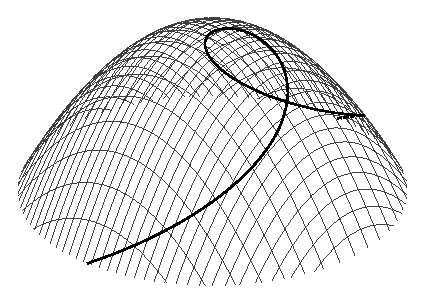
\includegraphics[width=8cm,height=8cm]{figures/parab}
  \end{center}

  \caption{\small Surface plotting with Gnuplot.}
  \label{fig-gnuplot}
\end{figure}

\lstset{frame=single, basicstyle=\small}
\mbox{
\lstinputlisting{figures/c_parabola}}


\section{Surfaces with \myindx{Google Sketchup}}
Google Sketchup is a 3D modelling tool provided free of charge. One cool 
feature of Sketchup is the API which makes it easy to write custom plugins 
for creating 3D graphics. In Sketchup we have fine control over colors, 
transparency, shadows, materials and because Sketchup is Polygon based it 
can also do hidden line removal. Put the following Ruby script in the Plugins 
folder and it will automatically run when you start Sketchup. The result is shown in figure \ref{fig-sketchup}.

\begin{figure}[!ht]
  \begin{center}
    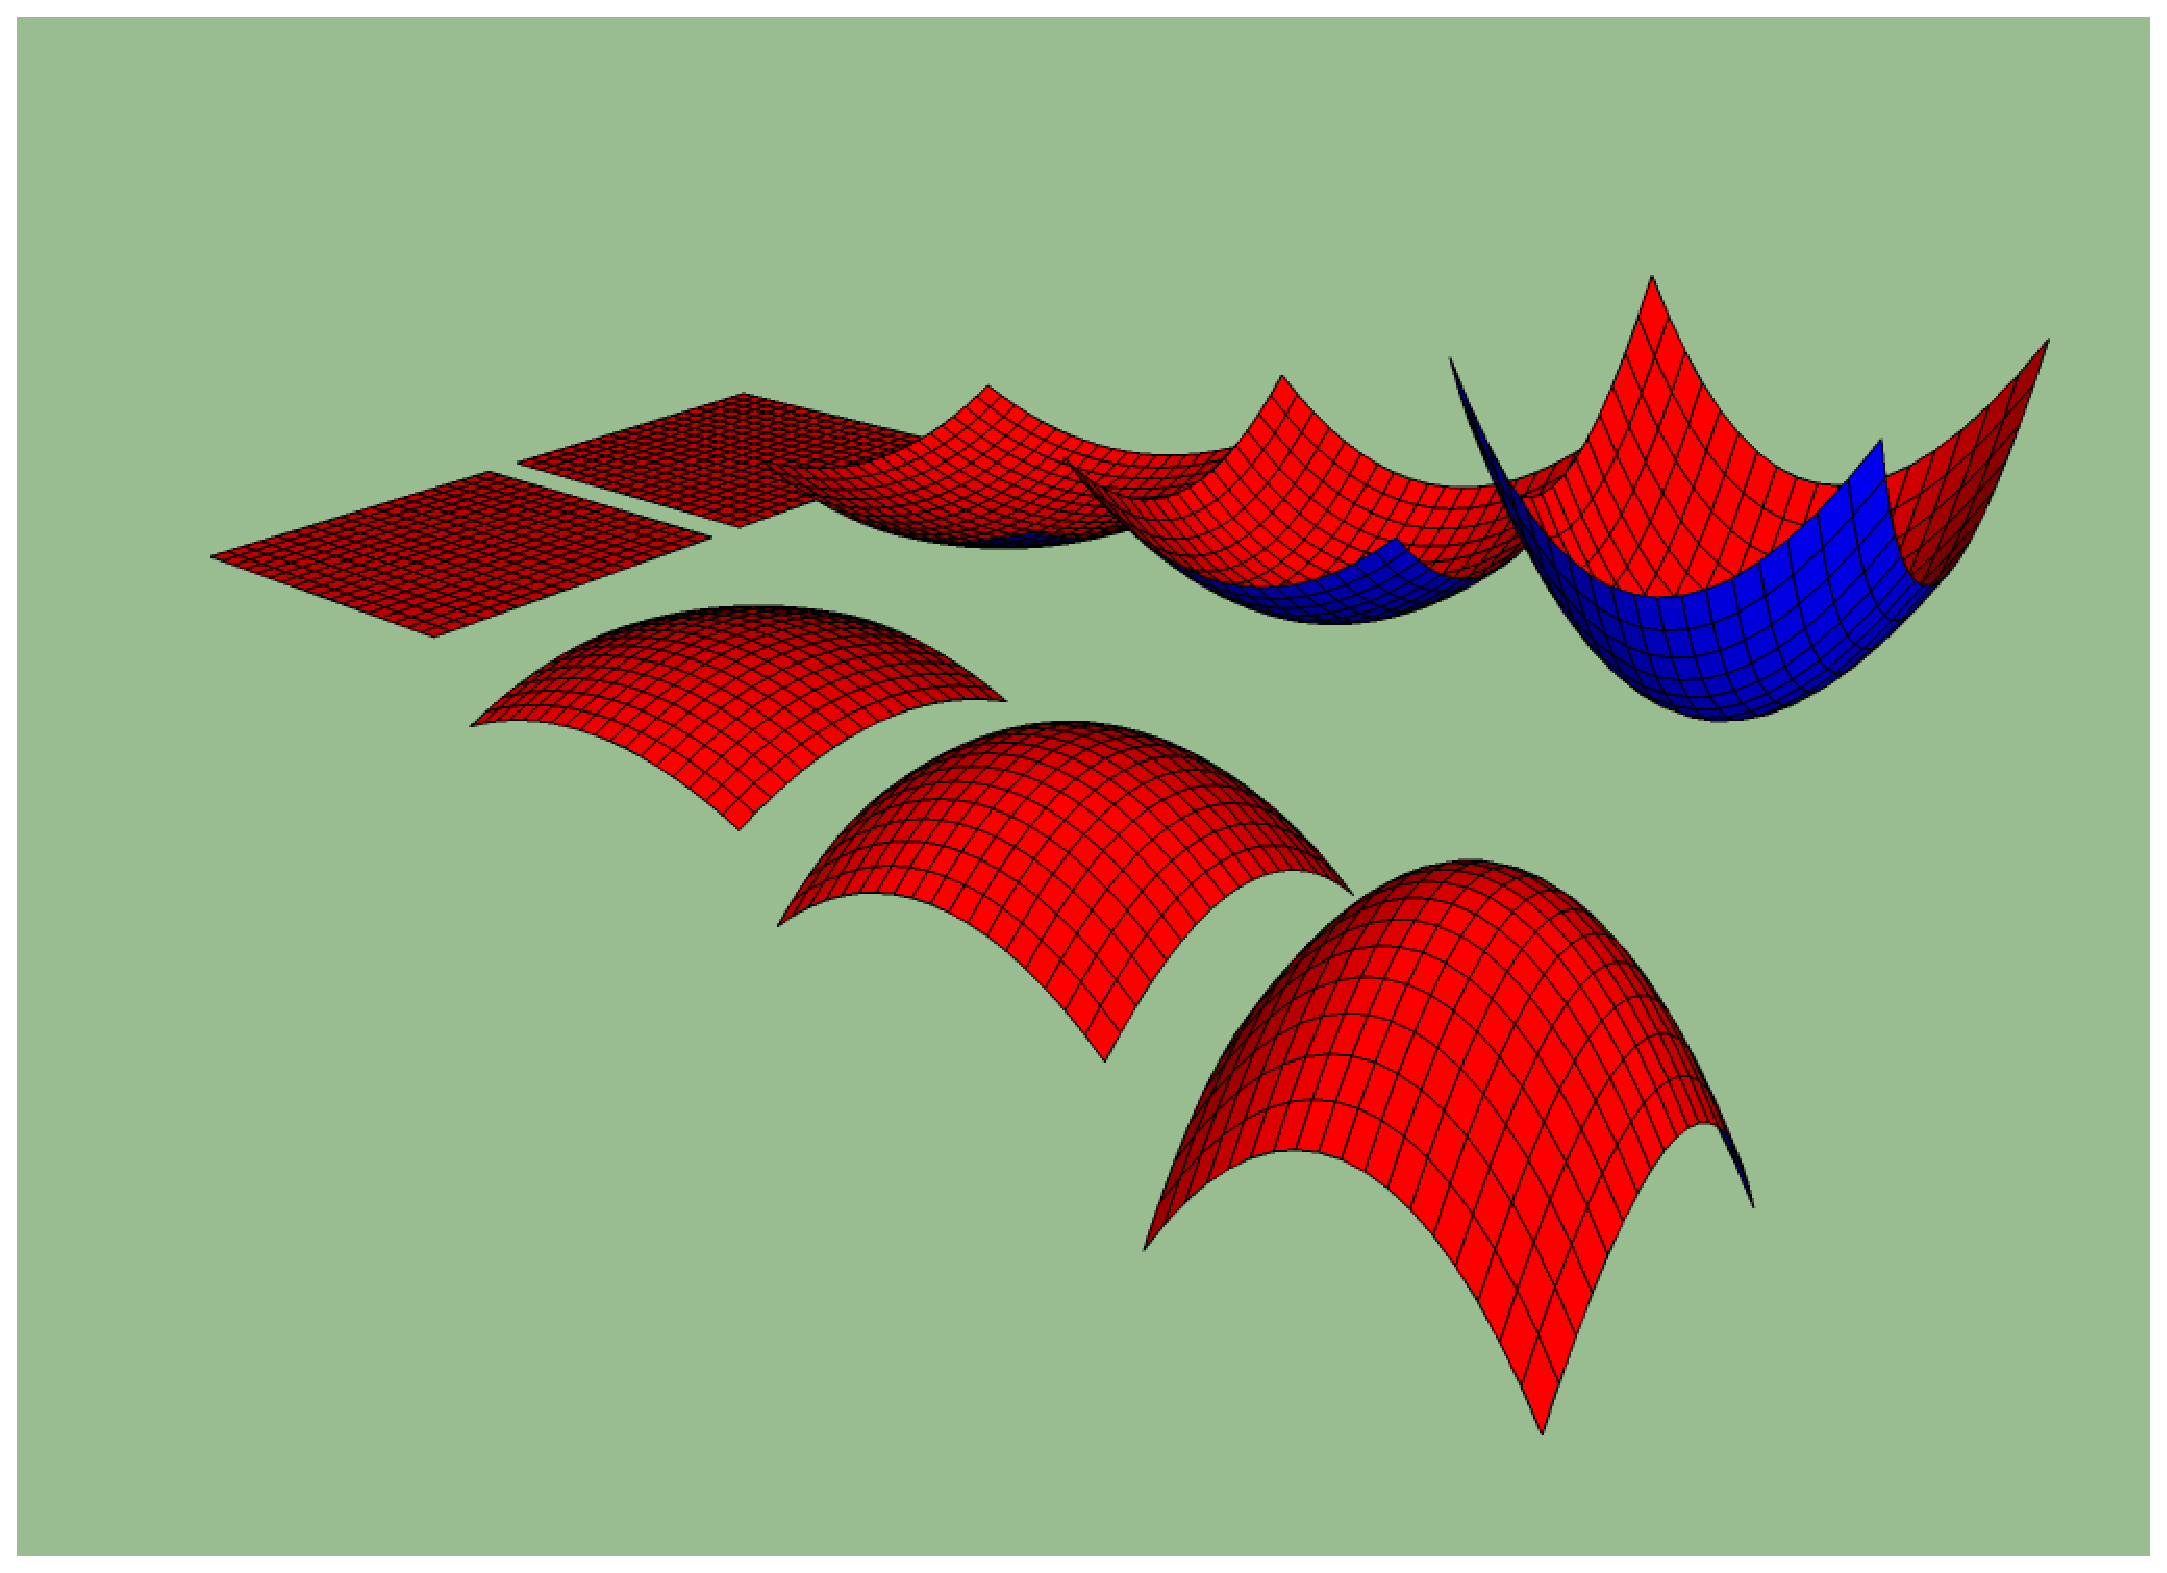
\includegraphics[width=12cm,height=12cm]{figures/rubyparabolas}
  \end{center}

  \caption{\small Plots generated by Google Sketchup plugin.}
  \label{fig-sketchup}
\end{figure}

\lstset{frame=single, basicstyle=\small}
\lstinputlisting{figures/parab.rb}


\section{\LaTeX, \myindx{\TikZ} and GNUPLOT}
If you feel the need for more graphical consistency in your mathematical
figures, you could use \TikZ which is a large framework for drawing graphics
within \LaTeX.

This ended up being my favorite because embedding the graphics allows
for a more coherent graphical representation with styles. Another 
advantage is that there is less hassle with including external 
plots and keeping these files up to date.

If The following lines of code are added to your document,



\begin{lstlisting}
  \begin{tikzpicture}[scale=2]
    \draw[step=.25cm,mjcgrid] (-0.74,-0.24) grid (3.4,2.4);
    \pgfsetlinewidth{1pt}

    \coordinate (o)  at (0,0);
    \coordinate (ox) at (3,0);
    \coordinate (oy) at (0,2);
    \draw [->] (o) -- (ox); 
    \draw [->] (o) -- (oy); 

    \node [right]  at (ox) {$\mathbf{x}$};
    \node [above]  at (oy) {$\mathbf{y}$};

    \draw[scale=0.5,domain=-3.141:3.141,smooth,red] 
          plot[parametric,prefix=pgffigs/mjc,id=par_test] 
          function{2+t*cos(t),1+t*sin(t)};
  \end{tikzpicture}
\end{lstlisting}

this figure will be produced. The key ``magic'' is the \textbf{draw ... plot} commands. 
\TikZ generates a gnuplot file, makes \LaTeX\ call GNUPLOT, which in turn generates
a file with a table of the computed values. These values are then read and presented 
in the graphical framework \TikZ produces.

\begin{center}
  \begin{tikzpicture}[scale=2]
    \draw[step=.25cm,mjcgrid] (-0.74,-0.24) grid (3.4,2.4);
    \pgfsetlinewidth{1pt}

    \coordinate (o)  at (0,0);
    \coordinate (ox) at (3,0);
    \coordinate (oy) at (0,2);
    \draw [->] (o) -- (ox); 
    \draw [->] (o) -- (oy); 

    \node [right]  at (ox) {$\mathbf{x}$};
    \node [above]  at (oy) {$\mathbf{y}$};

    \draw[scale=0.5,domain=-3.141:3.141,smooth,red] plot[parametric,prefix=pgffigs/mjc,id=par_test] 
            function{2+t*cos(t),1+t*sin(t)};
  \end{tikzpicture}
\end{center}


\section{Numerical integration}
For definite integrals of functions of one variable, \myindx{Romberg integration} was used. The program 
listed below is compiled and executed by the following commands

\command{gcc romberg.c} 

\command{./a.out}


\lstset{frame=single, basicstyle=\tiny}
\lstinputlisting{numerical/romberg.c}


\section{\myindx{Symbolic algebra} with Maxima}
\label{sec:maxima}

The following code written in Maxima, produces the output in section \ref{sec:maxima_sph}

\begin{lstlisting}
   load(ctensor);

   ct_coordsys([r*cos(theta)*cos(phi),r*cos(theta)*sin(phi),
      r*sin(theta),[r,theta,phi]]);

   lg:trigsimp(lg);

   christof(lcs);

   ug:invert(lg);

   christof(mcs);
\end{lstlisting}


  
\newcommand{\addbib}[4]{
   \bibitem{#1} #2 \textbf{``\emph{#3}''}, #4
}

\begin{thebibliography}{99}

   \addbib{berry}{M.V. Berry}{Principles of Cosmology and Gravitation}{Adam Hilger}
   \addbib{dunham}{W. Dunham}{Euler, The master of us all}{The Mathematical Association of America}
   \addbib{einstein}{A. Einstein}{Relativity, the special and general theory}{Crown Publishers Inc.}
   \addbib{night}{J. Foster and D.J. Nightingale}{A Short Course in General Relativity}{Springer-Verlag New York Inc.;  2nd Revised edition}
   \addbib{gauss}{D. Kehlmann}{Measuring the World}{Pantheon Books}
   \addbib{misner}{C.W. Misner, K.S. Thorne and J.A. Wheeler}{GRAVITATION}{W.H. Freeman and Company}
   \addbib{latex}{T. Oetiker et al.}{The not so Short Introduction to \LaTeXe}{ }
   \addbib{padman}{T. Padman}{GRAVITATION Foundations and Frontiers}{Cambridge University Press}
   \addbib{recipes}{W.H. Press, S.A. Teukolsky, V.T. Vetterling and B.P. Flanagan}{Numerical Recipes 3rd Edition: The Art of Scientific Computing}{ Cambridge University Press }
   \addbib{maxima}{W. Schelter et al.}{Maxima Computer Algebra System}{\url{www.maxima-project.org}}
   \addbib{art:tiwari}{R.K. Tiwari, F. Rahaman and S. Ray}{Five Dimensional Cosmological Models in General Relativity}{Int.J.Theor.Phys.49:2348-2357,2010}
   \addbib{tikz}{T. Tantau}{The Ti\emph{k}Z and PGF Packages}{Institut F\"ur Teoretische Informatik, Universit\"at zu L\"ubeck }

\end{thebibliography}

  \printindex

\enlargethispage{3\baselineskip}
\thispagestyle{empty}
\pagecolor[HTML]{660066}

\begin{center}
\begin{minipage}{.9\textwidth}
\color{white}\Large\bfseries
This pamphlet started as a self study in General Relativity, a subject along with 
Astronomy which have inspired me over the years. However, in order to (as far as I can) completely
understand the subject of GR I really had to read up on the mathematics of 
curved surfaces.


\begin{center}
\LARGE\bfseries\sffamily\color{yellow}`Not too bad.' - A. Nonymous
\end{center}

I then decided to wrap up my notes so I could pick up where I left at some later 
time. For typesetting I reverted back to one of my old favorites - \LaTeX - and 
investigated what was new since I wrote my Ph.D. fifteen years ago. I then 
found the TikZ package which was very suitable for presenting some nice graphics.
So here we are - enjoy!

\end{minipage}
\end{center}

\vspace*{\stretch{1}}

\begin{center}
\vspace*{\baselineskip}

\textbf{\textcolor{white}{jCAPS Publishing \textbullet\ \texttt{http://www.jcaps.com}}}

\textbf{\textcolor{yellow}{Forsidedesign af Morten Jagd Christensen \textbullet\ \texttt{http://www.jcaps.com}}}

\vspace{0.25cm}
\includegraphics[width=40mm]{figures/jcapslogo.jpg}
\end{center}

\vspace{1.25cm}

\begin{minipage}{0.5\textwidth}
\colorbox{white}{\EANisbn[SC4]}
\end{minipage}



\end{document}
